\documentclass[UTF8,fontset=none,a4paper,11pt]{ctexart}

\usepackage{fontspec}
\usepackage{xeCJK}
\setCJKmainfont{Noto Serif CJK SC}[BoldFont={Noto Serif CJK SC Bold}]
\setCJKsansfont{Noto Sans CJK SC}[BoldFont={Noto Sans CJK SC Bold}]
\setCJKmonofont{Noto Sans Mono CJK SC}
\setmonofont{Noto Sans Mono CJK SC}

% ---------------------------------------------------------------------------
% Packages
% ---------------------------------------------------------------------------
\usepackage{geometry}
\geometry{left=2.6cm,right=2.6cm,top=2.6cm,bottom=2.6cm,headsep=0.7cm}
\usepackage{graphicx}
\usepackage{xcolor}
\usepackage{booktabs}
\usepackage{tabularx}
\usepackage{array}
\usepackage{longtable}
\usepackage{enumitem}
\usepackage{amsmath,amssymb}
\usepackage{tcolorbox}
\tcbuselibrary{listings,skins,breakable}
\usepackage{listings}
\usepackage{fancyhdr}
\usepackage{float}
\usepackage{needspace}
\usepackage{xurl}
\usepackage{tikz}
\usetikzlibrary{arrows.meta,positioning,fit,backgrounds,shapes.geometric,calc}

\definecolor{linkblue}{HTML}{1F5FA8}
\definecolor{codebg}{HTML}{F6F8FA}
\definecolor{codeframe}{HTML}{D0D7DE}
\definecolor{noteblue}{HTML}{2F6FB0}
\definecolor{tipgreen}{HTML}{2E7D4F}
\definecolor{warnred}{HTML}{B23A2E}

\usepackage[colorlinks=true,linkcolor=linkblue,urlcolor=linkblue,citecolor=linkblue,
  bookmarksnumbered=true,pdfencoding=auto,
  pdftitle={为 Deep Learning Club 学习教程做贡献：零基础指南},
  pdfsubject={面向第一次参与 Ulink 深度学习社讲义项目的零基础贡献指南},
  pdfkeywords={贡献指南, Git, GitHub, Markdown, MyST, 深度学习}]{hyperref}

\graphicspath{{img/}}

% ---------------------------------------------------------------------------
% Layout
% ---------------------------------------------------------------------------
\linespread{1.25}
\setlength{\headheight}{13pt}
\setcounter{secnumdepth}{2}
\setcounter{tocdepth}{2}
\setlength{\parindent}{2em}

\ctexset{
  section    = {format = \Large\bfseries\sffamily},
  subsection = {format = \large\bfseries\sffamily},
}

\pagestyle{fancy}
\fancyhf{}
\fancyhead[L]{\small\sffamily 为 Deep Learning Club 学习教程做贡献}
\fancyhead[R]{\small\sffamily\nouppercase{\leftmark}}
\fancyfoot[C]{\thepage}
\renewcommand{\headrulewidth}{0.4pt}

% ---------------------------------------------------------------------------
% Helpers
% ---------------------------------------------------------------------------
\newcommand{\code}[1]{{\CJKsetecglue{}\ttfamily #1}}
\newcommand{\bk}{\textasciigrave}
\newcommand{\chk}{\item[{\small$\boxtimes$}]}

\newcolumntype{L}[1]{>{\raggedright\arraybackslash}p{#1}}
\newcolumntype{Y}{>{\raggedright\arraybackslash}X}

% Admonitions (Quarkdown note / tip / warning)
\newtcolorbox{notebox}[1]{
  enhanced,breakable,
  colback=noteblue!4!white,colframe=noteblue,
  colbacktitle=noteblue,coltitle=white,
  fonttitle=\bfseries\sffamily,
  boxrule=0.6pt,arc=2pt,
  left=7pt,right=7pt,top=5pt,bottom=5pt,
  title={#1}
}
\newtcolorbox{tipbox}[1]{
  enhanced,breakable,
  colback=tipgreen!4!white,colframe=tipgreen,
  colbacktitle=tipgreen,coltitle=white,
  fonttitle=\bfseries\sffamily,
  boxrule=0.6pt,arc=2pt,
  left=7pt,right=7pt,top=5pt,bottom=5pt,
  title={#1}
}
\newtcolorbox{warnbox}[1]{
  enhanced,breakable,
  colback=warnred!4!white,colframe=warnred,
  colbacktitle=warnred,coltitle=white,
  fonttitle=\bfseries\sffamily,
  boxrule=0.6pt,arc=2pt,
  left=7pt,right=7pt,top=5pt,bottom=5pt,
  title={#1}
}

% Code blocks
\lstdefinestyle{qdstyle}{
  basicstyle=\ttfamily\small,
  keywordstyle=\color{linkblue!80!black}\bfseries,
  commentstyle=\color{black!55},
  stringstyle=\color{tipgreen!80!black},
  breaklines=true,
  breakatwhitespace=false,
  columns=fullflexible,
  keepspaces=true,
  showstringspaces=false,
  backgroundcolor=\color{codebg},
  frame=single,
  rulecolor=\color{codeframe},
  framerule=0.4pt,
  framesep=4pt,
  xleftmargin=2pt,
  xrightmargin=2pt,
  aboveskip=10pt,
  belowskip=10pt,
  tabsize=2,
}
\lstset{style=qdstyle}

% Flowchart styles
\tikzset{
  flow/.style={draw=black!60,fill=blue!3,rounded corners=2.5pt,align=center,
    inner sep=5pt,font=\small\sffamily,minimum height=0.85cm},
  flowin/.style={flow,fill=green!6},
  flowout/.style={flow,fill=orange!8},
  flow6/.style={flow,font=\footnotesize\sffamily,inner sep=4pt},
  decision/.style={draw=black!60,fill=yellow!10,diamond,aspect=2.1,align=center,
    inner sep=1pt,font=\small\sffamily},
  edge/.style={-{Stealth[length=2mm]},draw=black!65,thick},
  elabel/.style={font=\scriptsize\sffamily,fill=white,inner sep=1.5pt},
  groupbox/.style={draw=black!30,dashed,rounded corners=5pt,fill=blue!1,inner sep=9pt},
}

% ---------------------------------------------------------------------------
\begin{document}

% ============================== Title page =================================
\begin{titlepage}
\centering
\vspace*{2.2cm}

{\sffamily\bfseries\Huge 为 Deep Learning Club 学习教程做贡献\par}
\vspace{0.35em}
{\sffamily\bfseries\Huge 零基础指南\par}

\vspace{1.4cm}
{\large 面向第一次参与 Ulink 深度学习社讲义项目的零基础贡献指南，\par}
{\large 涵盖 Git 流程、Markdown 与 MyST 写法。\par}

\vspace{1.6cm}
{\large 项目仓库：\href{https://github.com/ulink-deep-learning-club/ulink-deeplearningclub-handouts}{ulink-deep-learning-club/\allowbreak ulink-deeplearningclub-handouts}\par}
\vspace{0.5em}
{\large 在线文档：\href{https://ulink-deep-learning-club.github.io/ulink-deeplearningclub-handouts/}{ulink-deep-learning-club.github.io/\allowbreak ulink-deeplearningclub-handouts}\par}

\vfill
{\large 关键词：贡献指南\quad Git\quad GitHub\quad Markdown\quad MyST\quad 深度学习\par}
\vspace{0.7cm}
{\large \today\par}
\end{titlepage}

% ================================== TOC ====================================
\tableofcontents
\thispagestyle{plain}
\clearpage

% ============================== 怎么用这份指南 =============================
\section*{怎么用这份指南}
\addcontentsline{toc}{section}{怎么用这份指南}
\markboth{怎么用这份指南}{}

\begin{center}
\small
\begin{tabularx}{\linewidth}{@{}L{5.2cm}Y@{}}
\toprule
你的情况 & 先读 \\
\midrule
先认识仓库页面 & 第~\ref{sec:project-layout}~节 \\
安装本地环境 & 第~\ref{sec:setup-tools}~节 \\
只想改一个错别字 & 第~\ref{sec:web-edit}~节 \\
第一次完整走 PR 流程 & 第~\ref{sec:setup-tools}、\ref{sec:full-workflow}~节 \\
要新增或改写章节 & 第~\ref{sec:full-workflow}、\ref{sec:myst-syntax}、\ref{sec:writing-rules}~节 \\
要改代码示例 & 第~\ref{sec:full-workflow}、\ref{sec:myst-syntax}、\ref{sec:code-contrib}~节 \\
要做英文翻译 & 第~\ref{sec:full-workflow}、\ref{sec:translation}~节 \\
遇到报错 & 第~\ref{sec:faq}~节 \\
\bottomrule
\end{tabularx}
\end{center}

\clearpage

% ============================== 1. 项目里有什么 ============================
\section{项目里有什么}\label{sec:project-layout}

仓库页面顶部有一排标签，它们负责不同操作，不是目录：

\begin{center}
\small
\begin{tabularx}{\linewidth}{@{}L{4.4cm}Y@{}}
\toprule
标签 & 用途 \\
\midrule
\code{Code} & 浏览文件、目录和提交历史。大部分时间在这里。 \\
\code{Issues} & 讨论问题和提出修改建议。 \\
\code{Pull requests} & 提交、审阅和合并修改。 \\
\code{Agents} & GitHub 的自动化代理入口，本课程用不到。 \\
\code{Actions} & 查看自动构建和部署结果。 \\
\code{Projects} & 项目看板，本课程用不到。 \\
\code{Security and quality} & 安全扫描和依赖提醒，普通贡献者用不到。 \\
\code{Insights} & 贡献者、提交和访问统计。 \\
\code{Settings} & 仓库设置，只有维护者会动。 \\
\bottomrule
\end{tabularx}
\end{center}

\begin{figure}[htbp]
  \centering
  
\includegraphics[width=\linewidth]{01-repo-header.png}
  \caption[GitHub 仓库页顶部的标签栏，包括 Code、Issues、Pull requests、Actions 等]{仓库页顶部的标签栏。贡献时最常用的是 Code、Issues 和 Pull requests。}
\end{figure}

点 \code{Code}，页面下方显示当前分支的文件和目录：

\begin{figure}[htbp]
  \centering
  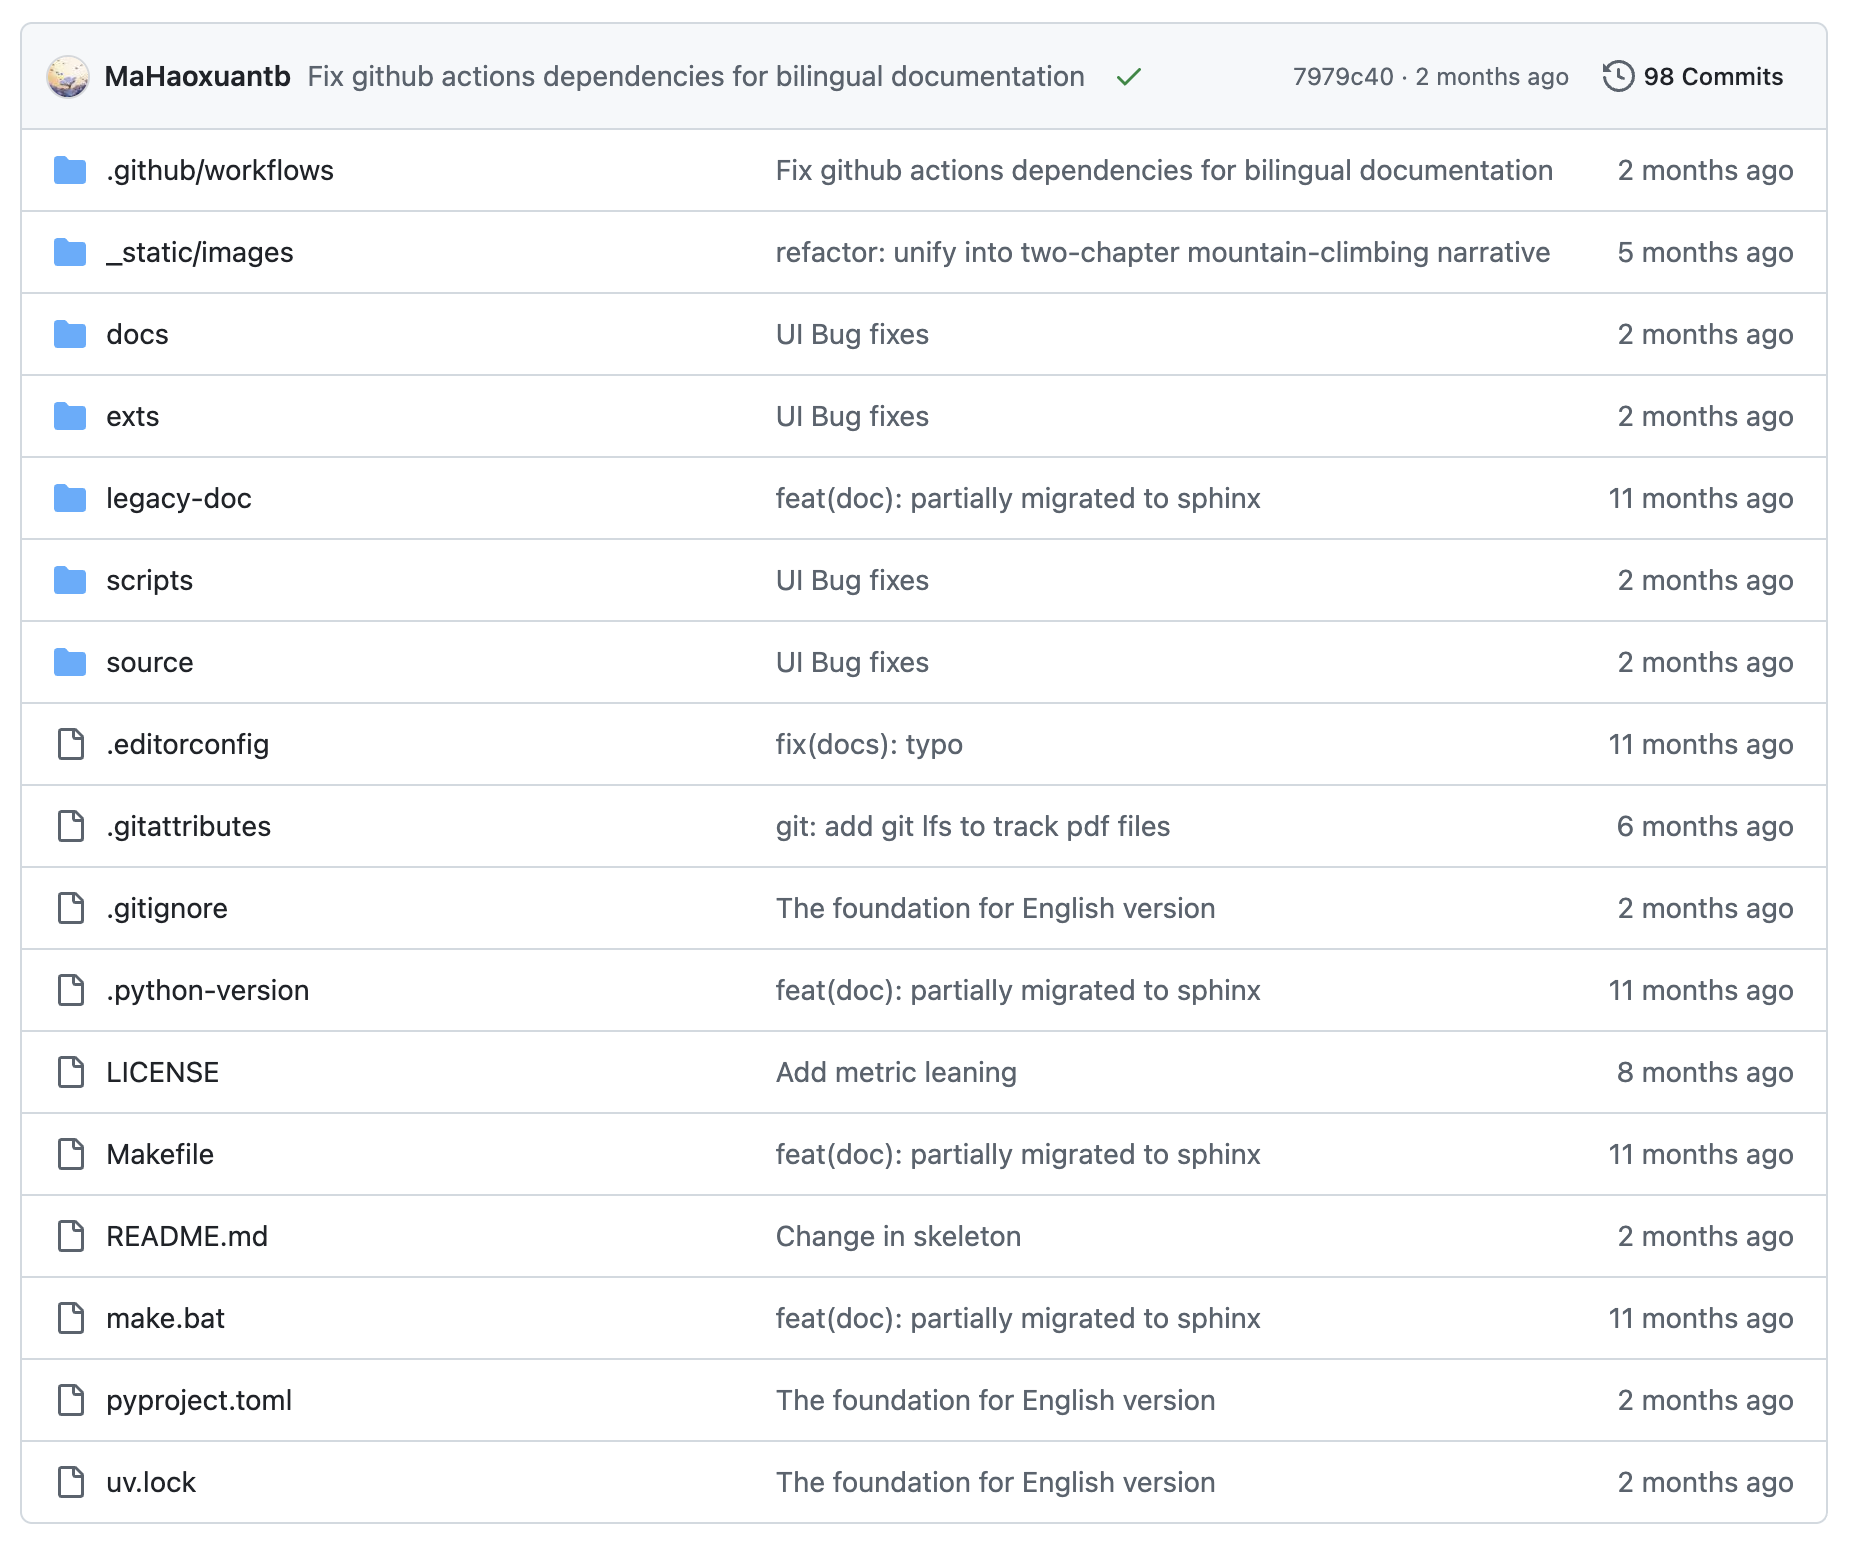
\includegraphics[width=\linewidth]{11-repo-files.png}
  \caption[Code 标签页下方的文件和目录列表，包括 docs、scripts、source 等]{Code 标签页下方的文件列表。目录名就是你在正文里引用的路径。}
\end{figure}

这些路径在 \code{Code} 标签页里都能看到，也都位于\href{https://github.com/ulink-deep-learning-club/ulink-deeplearningclub-handouts}{项目仓库}的 \code{main} 分支：

\begin{center}
\small
\begin{tabularx}{\linewidth}{@{}L{6.2cm}L{5.2cm}Y@{}}
\toprule
路径 & 内容 & 你需要动它吗 \\
\midrule
\code{source/} & 课程正文，按章节分目录 & 会，大部分修改在这里 \\
\code{source/\allowbreak appendix/\allowbreak sphinx-guide/\allowbreak index.md} & MyST 语法参考 & 写文档时查 \\
\code{source/references.bib} & 全局参考文献 & 加引用时动 \\
\code{source/\allowbreak locale/\allowbreak en/\allowbreak LC\_MESSAGES/} & 英文翻译目录（\code{.po}） & 做翻译时动 \\
\code{docs/} & 开发说明和本地化指南 & 查，不常改 \\
\code{scripts/} & 构建和中英文检查脚本 & 一般不动 \\
\code{legacy-doc/} & 已归档的 LaTeX 文档 & 不要动 \\
\code{build/}、\code{.venv/}、\code{cache/} & 编译产物和虚拟环境 & 不要提交 \\
\bottomrule
\end{tabularx}
\end{center}

大部分改动集中在 \code{source/}。点进去会看到 \code{math-fundamentals/}、\newline\code{cnn-expedition/}、\allowbreak\code{pytorch-practice/} 等章节目录，每个目录里通常有 \code{index.md}、若干内容文件和 \code{the-end.md}。

正文源文件只有一份，就是 \code{source/} 下的中文 Markdown。网页、PDF 和英文版都从它生成：

\begin{figure}[H]
  \centering
  \begin{tikzpicture}
    \node[flowin] (A) at (0,0) {source/ 中的 Markdown\\MyST 语法};
    \node[flow] (B) at (5.4,0) {Sphinx 编译};
    \node[flowout] (C) at (10.2,1.8) {HTML 网页};
    \node[flowout] (D) at (10.2,0) {PDF 电子书};
    \node[flowout] (E) at (10.2,-1.8) {EPUB 电子书};
    \node[flow] (F) at (2.7,-2.5) {gettext 目录\\source/locale/en};

    \draw[edge] (A) -- (B);
    \draw[edge] (B.east) -- ++(0.8,0) |- (C.west);
    \draw[edge] (B) -- (D);
    \draw[edge] (B.east) -- ++(0.8,0) |- (E.west);
    \draw[edge] (A.south) -- (A.south |- F.west) -- (F.west);
    \draw[edge] (F.east) -- (F.east -| B.south) -- (B.south);
  \end{tikzpicture}
  \caption{唯一的内容源与三种输出格式}
\end{figure}

编译后的网页长这样：

\begin{figure}[htbp]
  \centering
  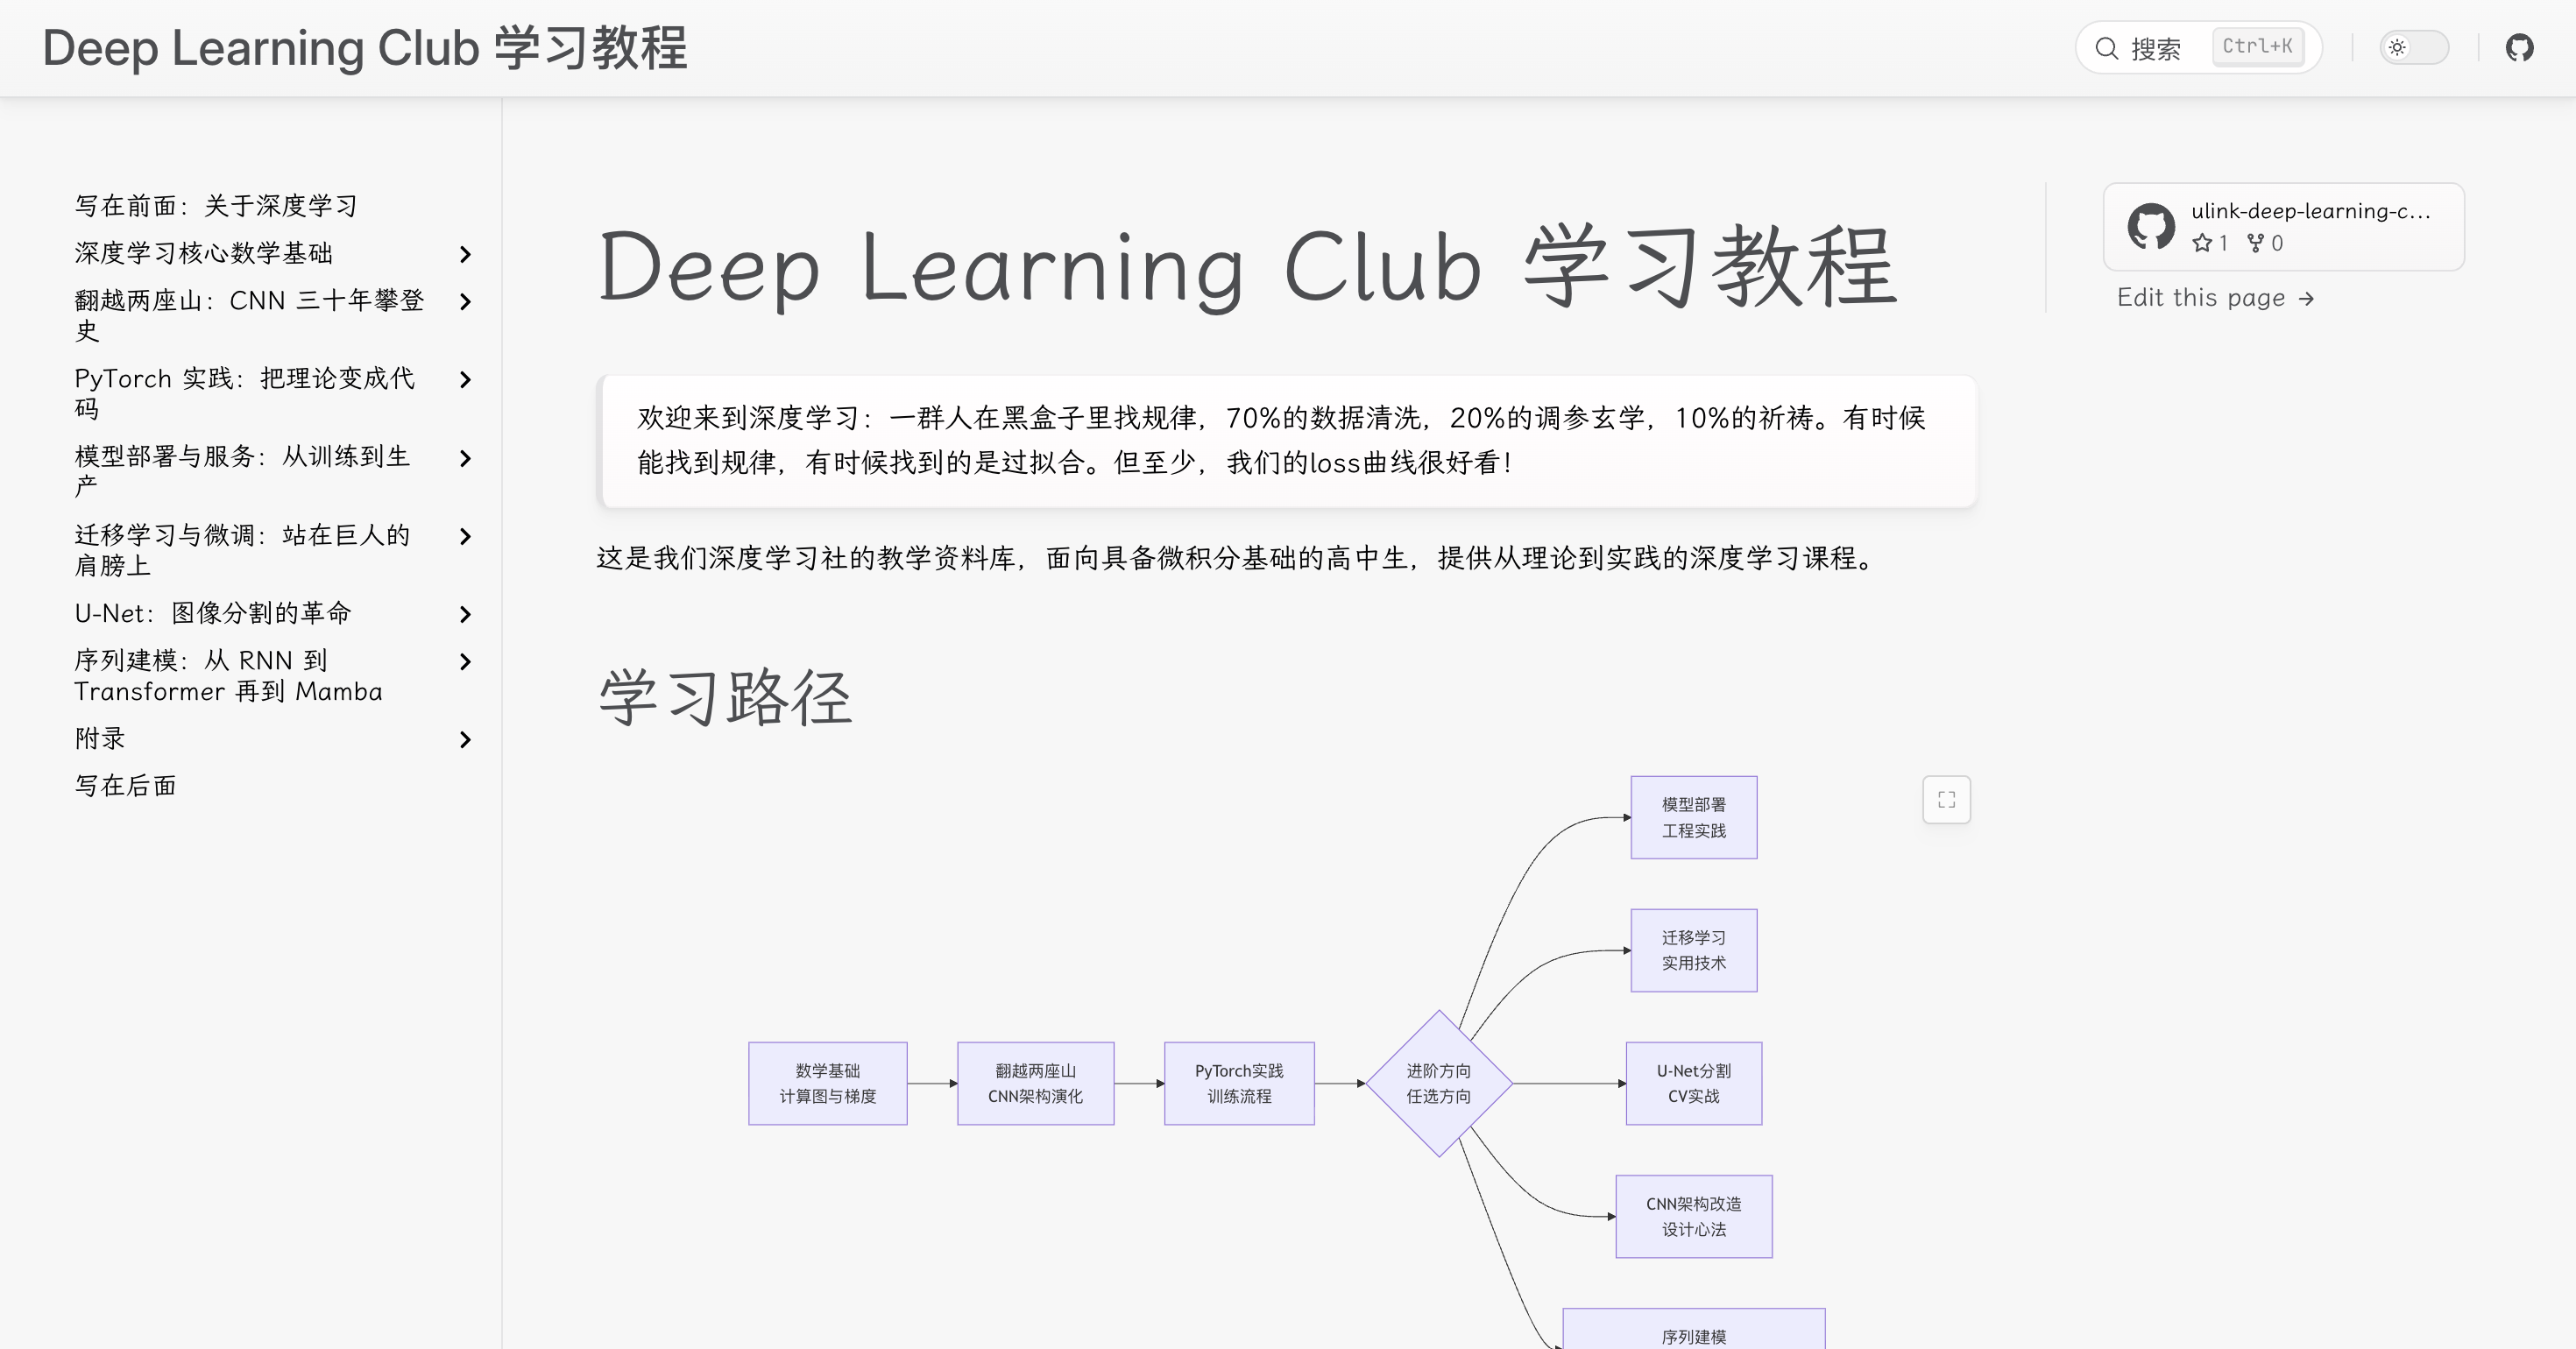
\includegraphics[width=\linewidth]{10-live-site.png}
  \caption[在线文档首页，左侧是章节目录，右侧是正文和 Mermaid 学习路径图]{编译后的在线文档。你改的是源文件，读者看到的是这个页面。}
\end{figure}

你改的是左边的源文件，读者看到的是编译后的页面。源文件里写错一个标签，编译时会出现警告，页面上的链接也可能断掉。

\clearpage

% ============================== 2. 四个词 ==================================
\section{四个词：仓库、分支、提交、PR}\label{sec:git-vocabulary}

Git 管的是文件的历史。你可以把它想成游戏存档：每次提交是一个存档点，分支是另一条存档线，合并就是把一条存档线接回主线。

你会接触两份仓库：

\begin{figure}[H]
  \centering
  \begin{tikzpicture}
    \node[flow] (U) at (0,0) {官方仓库 upstream\\ulink-deep-learning-club/...};
    \node[flow] (F) at (5.6,0) {你的 fork origin\\github.com/你的用户名/...};
    \node[flow] (L) at (11.2,0) {你的电脑\\本地仓库};
    \node[flowout] (W) at (0,-2.6) {在线文档\\gh-pages 分支};

    \draw[edge] (U) -- node[elabel]{Fork} (F);
    \draw[edge] (F) -- node[elabel]{git clone} (L);
    \draw[edge] (L.south) to[out=-120,in=-60] node[elabel,below]{git push} (F.south);
    \draw[edge] (F.north) to[out=120,in=60] node[elabel,above]{Pull Request} (U.north);
    \draw[edge] (U) -- node[elabel,right]{GitHub Actions} (W);
  \end{tikzpicture}
  \caption{官方仓库、你的 fork 与本地仓库的关系}
\end{figure}

\begin{center}
\small
\begin{tabularx}{\linewidth}{@{}L{3.4cm}YL{5.2cm}@{}}
\toprule
词 & 意思 & 在本项目里对应什么 \\
\midrule
仓库 repository & 一个带历史记录的项目目录 & 整个讲义 \\
Fork & 在 GitHub 上复制一份别人的仓库到你的账号 & 你的个人副本 \\
分支 branch & 仓库里一条独立的修改线 & \code{fix/typo-preface} 这类名字 \\
提交 commit & 一次有说明的修改记录 & 改完一段话后的存档 \\
远程 remote & 另一份仓库的地址 & \code{origin} 和 \code{upstream} \\
Pull Request (PR) & 请求官方仓库合并你的分支 & 审核和合并的地方 \\
Issue & 讨论问题或提出修改建议的帖子 & 动手前先对齐方向 \\
\bottomrule
\end{tabularx}
\end{center}

\code{origin} 指向你的 fork，你往这里推送。\code{upstream} 指向官方仓库，你从这里拉取最新内容。两个名字只是约定，但项目里的命令都按这个约定写。

文件从编辑到进入历史，会经过这几个位置：

\begin{figure}[H]
  \centering
  \begin{tikzpicture}[scale=0.95,transform shape]
    \node[flow6] (W) at (0,0) {工作区\\正在编辑的文件};
    \node[flow6] (S) at (4.4,0) {暂存区\\准备提交的改动};
    \node[flow6] (R) at (8.8,0) {本地仓库\\提交历史};
    \node[flow6] (O) at (13.2,0) {origin\\你的 fork};
    \node[flow6] (V) at (13.2,-2.7) {审阅和 CI};
    \node[flow6,fill=orange!8] (P) at (7.4,-2.7) {upstream\\官方仓库 main};

    \draw[edge] (W) -- node[elabel]{git add} (S);
    \draw[edge] (S) -- node[elabel]{git commit} (R);
    \draw[edge] (R) -- node[elabel]{git push} (O);
    \draw[edge] (O) -- node[elabel,right]{Pull Request} (V);
    \draw[edge] (V) -- node[elabel,above]{通过并合并} (P);
    \draw[edge] (P.west) -- node[elabel,above,midway]{git pull upstream main} (-0.9,-2.7) -- ($(W.south)+(-0.9,0)$);
    \draw[edge] (V.south) -- (13.2,-5.2) -- node[elabel,above,midway]{需要修改} (0.9,-5.2) -- ($(W.south)+(0.9,0)$);
  \end{tikzpicture}
  \caption{一次修改从工作区到合并的位置变化}
\end{figure}

分支在历史里是这样分开又合回来的：

\begin{figure}[H]
  \centering
  \begin{tikzpicture}[x=1.7cm,y=1cm,font=\scriptsize\sffamily]
    % main line
    \draw[thick,black!65] (0,0) -- (8.2,0);
    \foreach \x/\n in {0/初始版本,1.2/补充数学基础,2.4/upstream/main,4.2/其他人合并的改动,6.0/另一处文档更新,7.3/PR 合并,8.2/后续章节更新}{
      \fill[black!75] (\x,0) circle (2.2pt);
      \node[above,rotate=45,anchor=south west] at (\x,0) {\n};
    }
    % branch
    \draw[thick,black!65,rounded corners=5pt] (2.4,0) -- (2.4,-1.5) -- (7.3,-1.5) -- (7.3,0);
    \foreach \x/\n in {3.4/修改错别字,5.0/根据审阅意见调整}{
      \fill[black!75] (\x,-1.5) circle (2.2pt);
      \node[below,rotate=45,anchor=north west] at (\x,-1.5) {\n};
    }
  \end{tikzpicture}
  \caption{分支的创建、提交与合并}
\end{figure}

GitHub 的分支页面可以查看当前有哪些分支：

\begin{figure}[htbp]
  \centering
  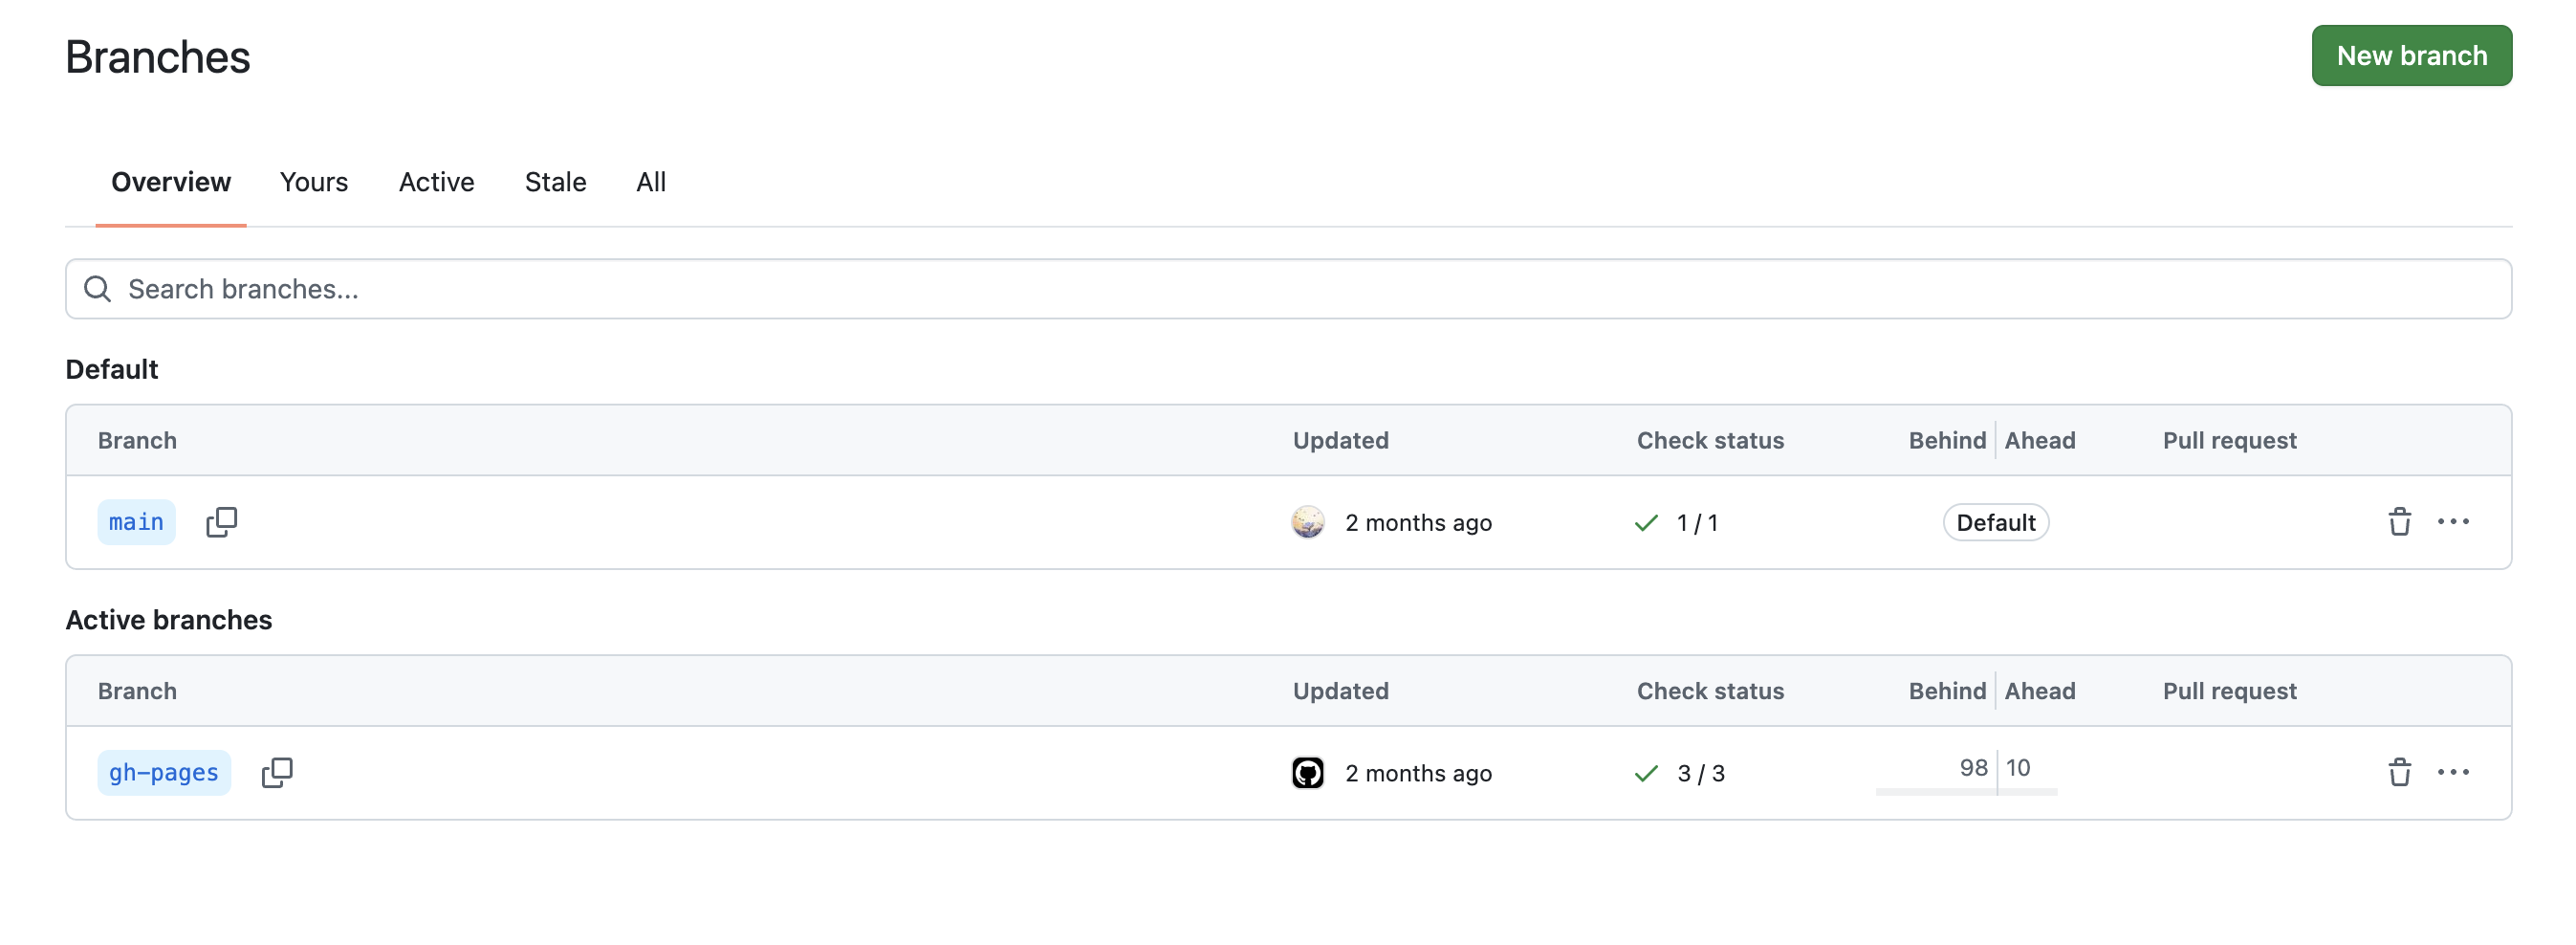
\includegraphics[width=\linewidth]{05-branches.png}
  \caption[GitHub Branches 页面，右上角有 New branch 按钮，列表中有 main 和 gh-pages]{分支页面。main 是默认分支，gh-pages 用来发布网页。}
\end{figure}

\clearpage

% ============================== 3. 装好工具 ================================
\section{装好工具}\label{sec:setup-tools}

最少需要 Git 和一个编辑器。构建网页还需要 Python 和 uv。画 Mermaid 图或生成 PDF 时，才需要 Node、Chromium 和 TeXLive。

\begin{center}
\small
\begin{tabularx}{\linewidth}{@{}L{3.8cm}L{4.8cm}Y@{}}
\toprule
工具 & 用途 & 检查命令 \\
\midrule
Git & 保存和同步修改 & \code{git --version} \\
GitHub 账号 & 托管 fork、Issue 和 PR & 浏览器登录 \\
编辑器 & 改 Markdown & VS Code、Zed、Cursor 都可以 \\
Python 3.13+ & 运行 Sphinx，版本以 \code{.python-version} 为准 & \code{python3 --version} \\
uv & 安装 Python 依赖 & \code{uv --version} \\
Node.js + mermaid-cli & 渲染 Mermaid & \code{mmdc --version} \\
TeXLive + pdf2svg & 生成 PDF 和 TikZ & \code{pdflatex --version} \\
\bottomrule
\end{tabularx}
\end{center}

Git 第一次使用要先写名字和邮箱：

\Needspace{5\baselineskip}
\begin{lstlisting}[language=bash]
git config --global user.name "你的名字"
git config --global user.email "你的邮箱"
\end{lstlisting}

这些信息会写进提交记录。邮箱用你愿意公开的那个。

\begin{tipbox}{Tip}
命令里的尖括号表示占位符，例如 \code{<文件>}。执行时换成真实内容，不要保留尖括号。
\end{tipbox}

macOS 可以用 Homebrew 安装：

\Needspace{5\baselineskip}
\begin{lstlisting}[language=bash]
brew install git uv node
npm install -g @mermaid-js/mermaid-cli
\end{lstlisting}

Windows 安装 \href{https://git-scm.com/download/win}{Git for Windows}，在 Git Bash 里执行文中的 bash 命令。本文用命令行；你也可以用 \href{https://desktop.github.com/}{GitHub Desktop} 完成同样的操作，但排错时命令更容易描述。

\code{uv} 的其他安装方式见\href{https://docs.astral.sh/uv/getting-started/installation/}{官方文档}。

Ubuntu 和 Debian 的完整依赖在\href{https://github.com/ulink-deep-learning-club/ulink-deeplearningclub-handouts/blob/main/source/appendix/build-docs.md}{本地构建说明}里。只改文字时不用装 TeXLive，\code{make html} 可以正常生成网页，缺少 Mermaid 或 TikZ 时对应图表不显示。

\clearpage

% ============================== 4. 网页上改错别字 ==========================
\section{最快的一次贡献：在网页上改一个错别字}\label{sec:web-edit}

如果只改一句话，可以完全不装 Git。打开官方仓库里的目标文件，点右上角的铅笔图标：

\begin{figure}[htbp]
  \centering
  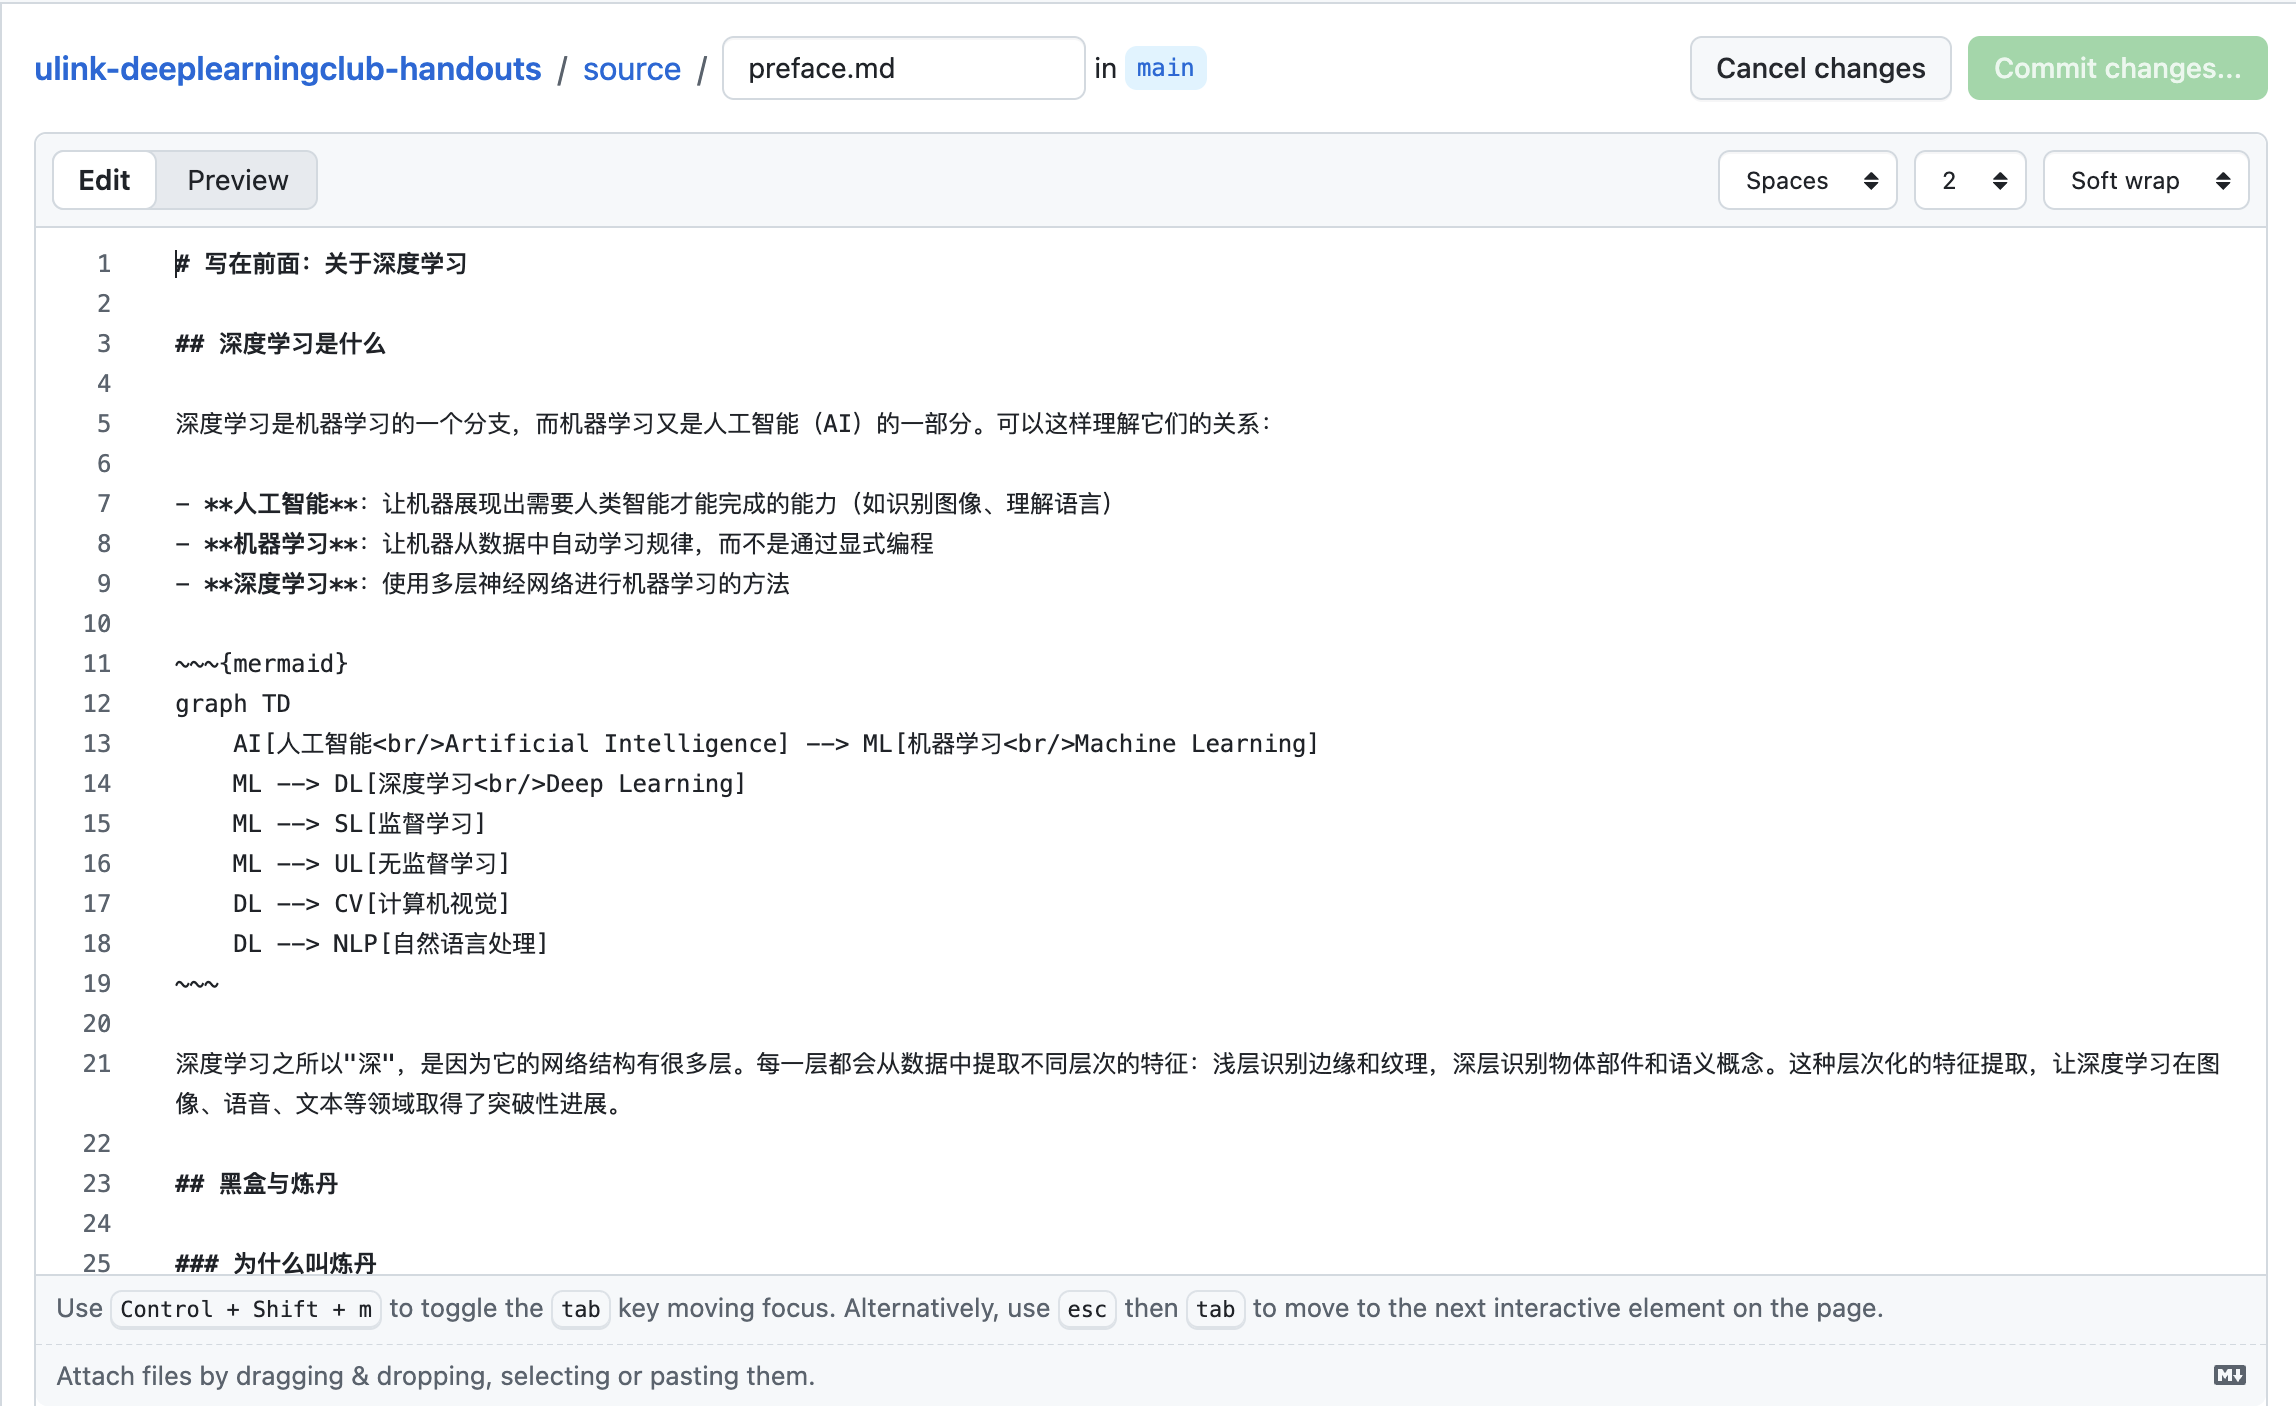
\includegraphics[width=0.78\linewidth]{06-edit-ui.png}
  \caption[GitHub 文件编辑页，顶部是文件路径和 Edit/Preview 标签，右上角是 Commit changes 按钮]{网页编辑器。改完可以切到 Preview 看格式，再点 Commit changes。}
\end{figure}

步骤是这样：

\begin{enumerate}[leftmargin=1.8em,itemsep=2pt]
  \item 在文件页面点铅笔图标，GitHub 会自动帮你 fork 一份。
  \item 在 \code{Edit} 里改文字，切到 \code{Preview} 看效果。
  \item 点 \code{Commit changes}。
  \item 选择 \code{Create a new branch for this commit and start a pull request}，给分支起名，例如 \code{fix/typo-preface}。
  \item 点 \code{Propose changes}，填写 PR 说明，再点 \code{Create pull request}。
\end{enumerate}

这条路径适合错别字、标点、一句话的语病。新增章节、改结构、加代码或做翻译时，用第~\ref{sec:full-workflow}~节的本地流程更方便，因为你能在提交前完整编译一次。

\clearpage

% ============================== 5. 完整流程 ================================
\section{完整流程：从 Issue 到合并}\label{sec:full-workflow}

\begin{figure}[H]
  \centering
  \begin{tikzpicture}[node distance=1.3cm and 0.8cm]
    % ---- prep group ----
    \node[flowin] (A) at (0,9.6) {发现问题或想加内容};
    \node[decision] (B) at (0,8.1) {改动大吗};
    \node[flow] (C) at (-3.0,6.5) {先开 Issue 讨论};
    \node[flow] (D) at (0,6.5) {直接修改};
    \node[flow] (E) at (0,5.1) {Fork 并 clone};
    \node[flow] (F) at (0,3.7) {从 upstream/main 新建分支};
    \node[flow] (G) at (0,2.3) {编辑 Markdown};

    % ---- ship group ----
    \node[flow] (H) at (7.4,9.6) {本地 make html 预览};
    \node[flow] (I) at (7.4,8.2) {git add 和 git commit};
    \node[flow] (J) at (7.4,6.8) {git push 到 origin};
    \node[flow] (K) at (7.4,5.4) {开 Pull Request};
    \node[flow] (L) at (7.4,4.0) {CI 检查和审阅};
    \node[flow] (M) at (7.4,2.6) {合并到 main};
    \node[flowout] (N) at (7.4,1.2) {自动部署到 gh-pages};

    % group boxes behind
    \begin{scope}[on background layer]
      \node[groupbox,fit=(A)(B)(C)(D)(E)(F)(G),
        label={[font=\small\bfseries\sffamily,text=black!70]above:准备与修改}] {};
      \node[groupbox,fit=(H)(I)(J)(K)(L)(M)(N),
        label={[font=\small\bfseries\sffamily,text=black!70]above:提交与合并}] {};
    \end{scope}

    % edges
    \draw[edge] (A) -- (B);
    \draw[edge] (B) -- node[elabel,right]{错别字或一句话} (D);
    \draw[edge] (B) -- node[elabel,above left]{新增章节、改结构、翻译} (C);
    \draw[edge] (C) -- (D);
    \draw[edge] (D) -- (E);
    \draw[edge] (E) -- (F);
    \draw[edge] (F) -- (G);

    \draw[edge] (H) -- (I);
    \draw[edge] (I) -- (J);
    \draw[edge] (J) -- (K);
    \draw[edge] (K) -- (L);
    \draw[edge] (L) -- node[elabel,right]{通过} (M);
    \draw[edge] (M) -- (N);
    \draw[edge] (L.west) -- (4.0,4.0) node[elabel,above,midway]{需要修改} -- (4.0,2.3) -- (G.east);
  \end{tikzpicture}
  \caption{从发现问题到部署上线的完整流程}
\end{figure}

\subsection{先开 Issue}\label{sec:issue-first}

项目约定先讨论再动手。错别字可以直接提 PR，其他改动建议先开 Issue，尤其是新增章节、删除内容、调整目录结构和翻译。

打开 \code{Issues}，点 \code{New issue}：

\begin{figure}[htbp]
  \centering
  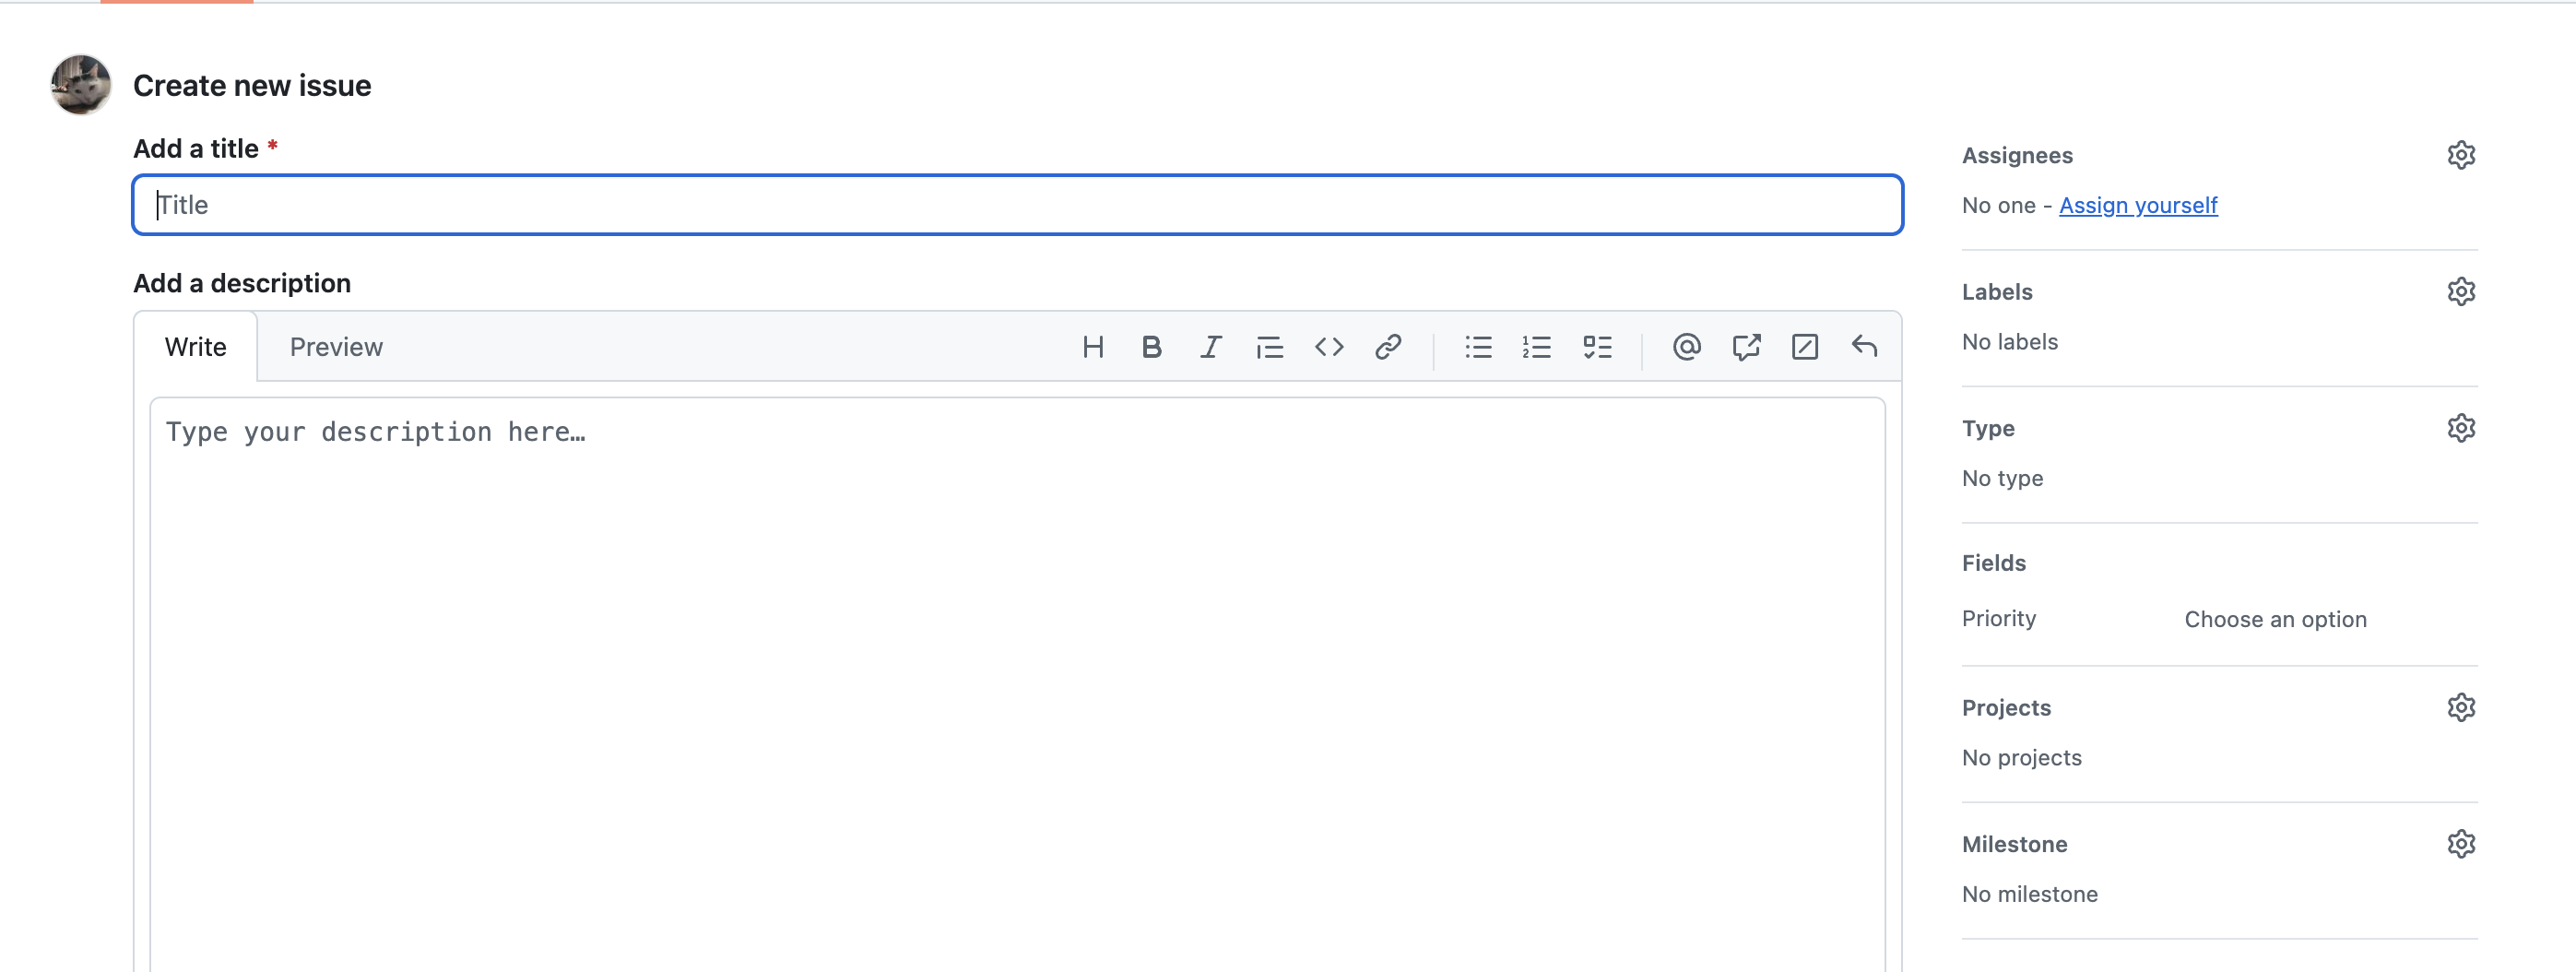
\includegraphics[width=\linewidth]{04-issue-form.png}
  \caption[GitHub 新建 Issue 页面，有标题输入框和描述编辑框]{新建 Issue。标题写类型和位置，正文写现状、建议和原因。}
\end{figure}

标题写清楚类型和位置，例如：

\Needspace{5\baselineskip}
\begin{lstlisting}
docs: 前言中的“机器学系”应为“机器学习”
\end{lstlisting}

正文可以按这个格式：

\Needspace{5\baselineskip}
\begin{lstlisting}
## 位置

`source/preface.md` 第 12 行

## 现在的内容

机器学系是人工智能的一个分支。

## 建议改成

机器学习是人工智能的一个分支。

## 原因

“机器学系”是错别字，读者会困惑。
\end{lstlisting}

\begin{warnbox}{Warning}
Issue 里不要放 API key、密码、个人身份信息或未公开的数据。需要贴截图时，先把无关的窗口和用户名遮掉。
\end{warnbox}

\subsection{Fork}\label{sec:fork}

打开官方仓库，点右上角的 \code{Fork}：

\begin{figure}[htbp]
  \centering
  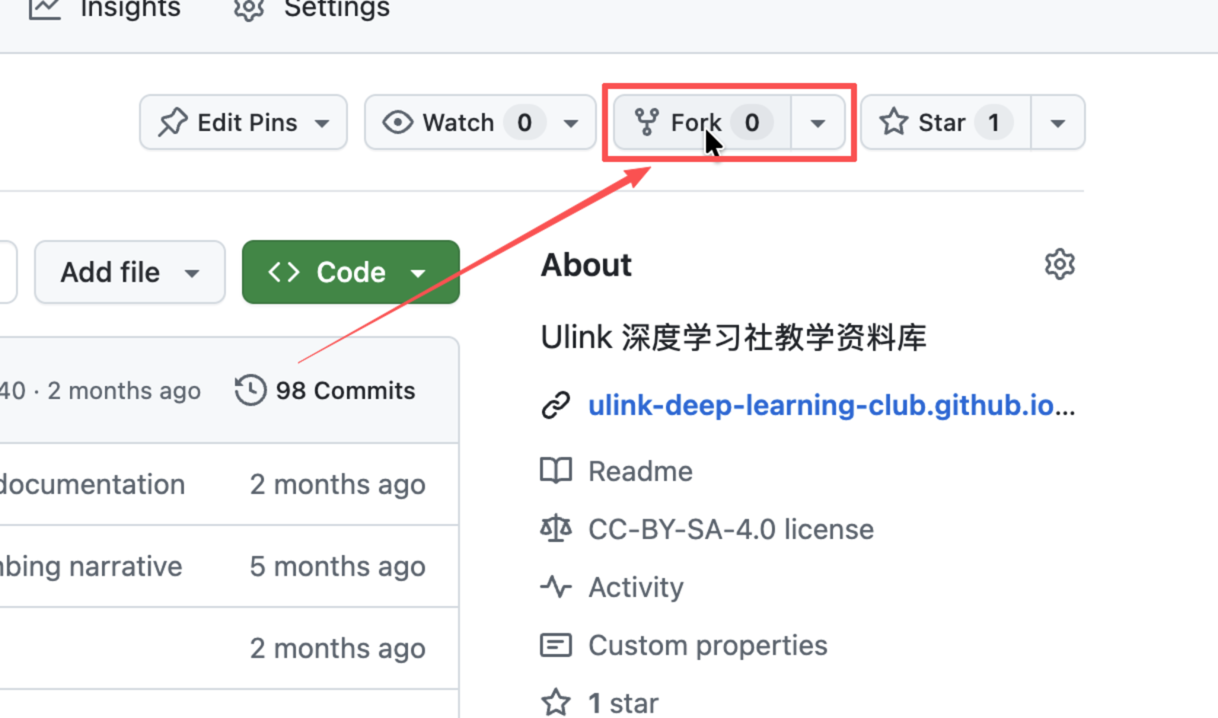
\includegraphics[width=0.62\linewidth]{03a-fork-btn.png}
  \caption[GitHub 仓库右上角的 Fork 按钮]{仓库右上角的 Fork 按钮。}
\end{figure}

GitHub 会打开创建 fork 的页面：

\begin{figure}[htbp]
  \centering
  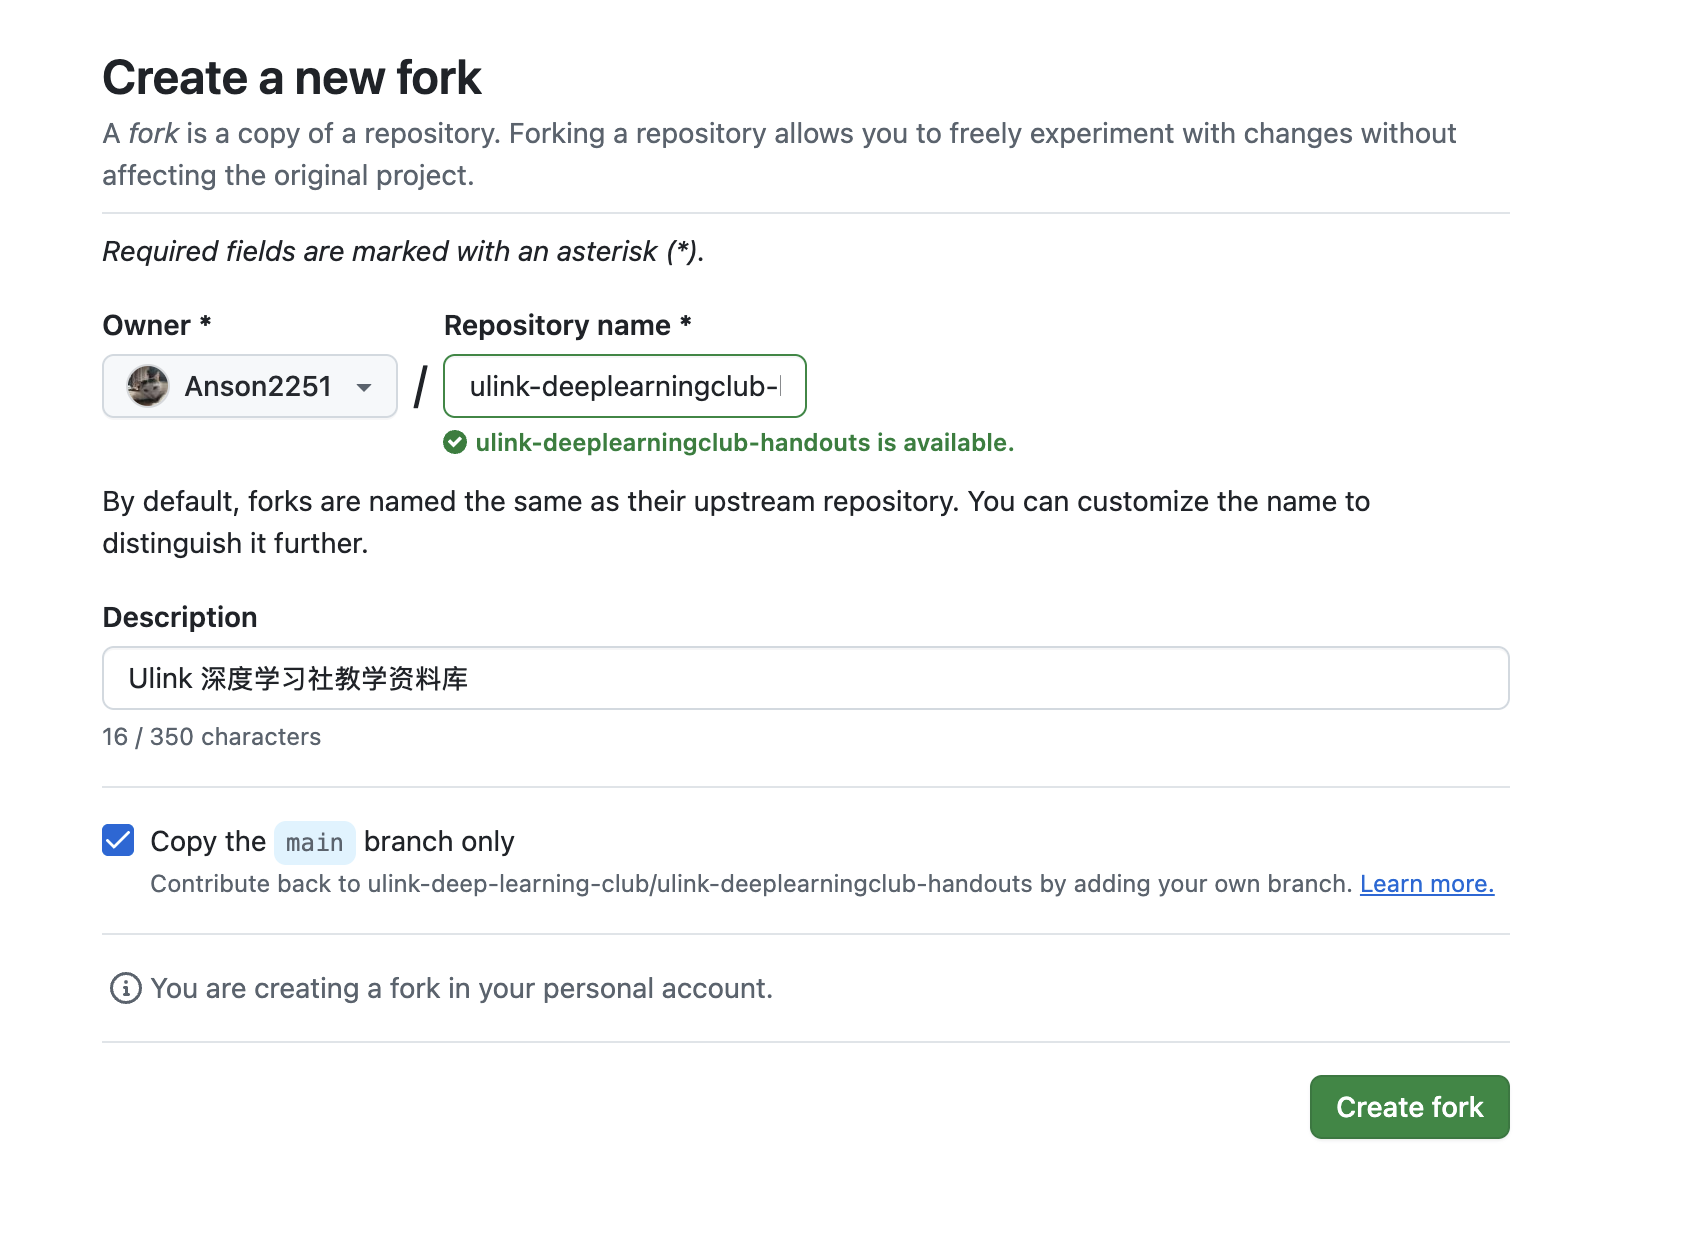
\includegraphics[width=0.75\linewidth]{03-fork-page.png}
  \caption[GitHub 创建 fork 页面，Owner 是你的账号，Repository name 默认与官方仓库同名，右下角是 Create fork]{创建 fork。Owner 选你的账号，名字保持默认，右下角点 Create fork。}
\end{figure}

保持默认名字，点 \code{Create fork}。完成后，你的账号下会有一份 \code{ulink-deeplearningclub-\allowbreak handouts}。

\subsection{Clone 到电脑}\label{sec:clone}

在你的 fork 页面点绿色的（示例中的 clone 菜单是官方仓库的，这里需要用你自己 fork 的仓库） \code{Code} 按钮，复制 HTTPS 地址：

\begin{figure}[htbp]
  \centering
  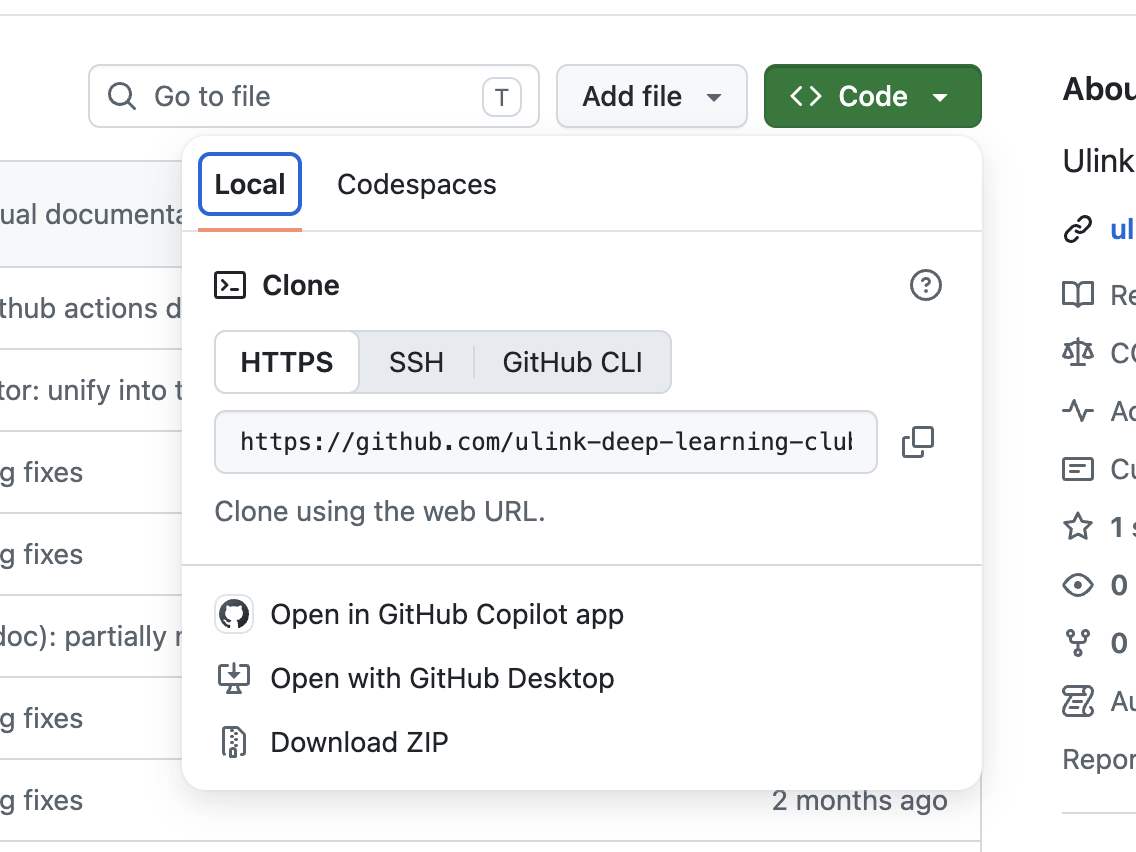
\includegraphics[width=0.62\linewidth]{02-clone-menu.png}
  \caption[GitHub Code 下拉菜单，HTTPS 标签下显示 clone 地址和复制按钮]{Code 菜单里的 HTTPS 地址，点右边的复制按钮。}
\end{figure}

然后在终端里执行下面的命令，把 \code{你的用户名} 换成你的 GitHub 用户名。

\Needspace{5\baselineskip}
\begin{lstlisting}[language=bash]
git clone https://github.com/你的用户名/ulink-deeplearningclub-handouts.git
cd ulink-deeplearningclub-handouts
\end{lstlisting}

把官方仓库添加为 \code{upstream}：

\Needspace{5\baselineskip}
\begin{lstlisting}[language=bash]
git remote add upstream https://github.com/ulink-deep-learning-club/ulink-deeplearningclub-handouts.git
git remote -v
\end{lstlisting}

\code{git remote -v} 应该显示四行，\code{origin} 两行指向你的 fork，\code{upstream} 两行指向官方仓库。如果提示 \code{remote upstream already exists}，说明已经加过了，不用重复加。地址不对时用：

\Needspace{5\baselineskip}
\begin{lstlisting}[language=bash]
git remote set-url upstream https://github.com/ulink-deep-learning-club/ulink-deeplearningclub-handouts.git
\end{lstlisting}

\subsection{安装依赖并预览}\label{sec:install-and-preview}

所有构建命令都在仓库根目录执行：

\Needspace{5\baselineskip}
\begin{lstlisting}[language=bash]
uv venv
uv sync
source .venv/bin/activate
make html
\end{lstlisting}

Windows PowerShell 的激活命令是：

\Needspace{5\baselineskip}
\begin{lstlisting}
.venv\Scripts\activate
\end{lstlisting}

Windows 上在 PowerShell 或 cmd 里运行 \code{make.bat html}，Git Bash 里没有 \code{make}。如果 \code{uv} 不可用，可以退回 Python 自带的虚拟环境：

\Needspace{5\baselineskip}
\begin{lstlisting}[language=bash]
python3 -m venv .venv
source .venv/bin/activate
python -m pip install -e .
make html
\end{lstlisting}

构建完成后启动本地服务器：

\Needspace{5\baselineskip}
\begin{lstlisting}[language=bash]
cd build/html
python -m http.server 8000 --bind 127.0.0.1
\end{lstlisting}

浏览器打开 \code{http://localhost:8000}。服务器会占用一个终端；改完源文件后，另开一个终端回到仓库根目录，再运行 \code{make html}，然后刷新浏览器就能看到变化。

如果你在 \code{build/html} 里迷路了，回到仓库根目录：

\Needspace{5\baselineskip}
\begin{lstlisting}[language=bash]
cd "$(git rev-parse --show-toplevel)"
\end{lstlisting}

只改中文正文时，\code{make html} 就够了。要检查中英文切换和 \code{/en/} 页面，用：

\Needspace{5\baselineskip}
\begin{lstlisting}[language=bash]
bash scripts/build-i18n-site.sh --html-only
\end{lstlisting}

\subsection{新建分支}\label{sec:new-branch}

不要直接在 \code{main} 上改，先从官方仓库拉最新内容，再开分支：

\Needspace{5\baselineskip}
\begin{lstlisting}[language=bash]
git fetch upstream
git switch -c fix/typo-preface upstream/main
\end{lstlisting}

分支名用能看懂的类型前缀：

\begin{center}
\small
\begin{tabularx}{\linewidth}{@{}L{2.2cm}L{3.6cm}Y@{}}
\toprule
前缀 & 用途 & 例子 \\
\midrule
\code{fix/} & 修错误 & \code{fix/typo-preface} \\
\code{docs/} & 文档调整 & \code{docs/clarify-backprop} \\
\code{feat/} & 新增内容 & \code{feat/lstm-section} \\
\code{i18n/} & 翻译 & \code{i18n/translate-preface} \\
\bottomrule
\end{tabularx}
\end{center}

\subsection{修改并检查}\label{sec:edit-and-check}

用编辑器打开文件。在 GitHub 文件页面按 \code{t} 可以打开文件搜索，或者点仓库首页的 \code{Go to file}。在本地不知道文字在哪个文件时，用 \code{git grep}：

\Needspace{5\baselineskip}
\begin{lstlisting}[language=bash]
git grep -n "机器学系"
\end{lstlisting}

它会输出文件名、行号和匹配内容。改完先看状态和差异：

\Needspace{5\baselineskip}
\begin{lstlisting}[language=bash]
git status
git diff
\end{lstlisting}

\code{git diff} 里，\code{-} 开头是删掉的内容，\code{+} 开头是新增的内容。提交前把整个 diff 读一遍，确认没有误删、没有把个人路径写进去、没有带进 \code{build/} 或 \code{.venv/}。

\subsection{提交}\label{sec:commit}

只添加你改过的文件：

\Needspace{5\baselineskip}
\begin{lstlisting}[language=bash]
git add source/preface.md
git commit -m "docs(preface): 修正“机器学系”错别字"
\end{lstlisting}

提交信息参考现有历史，格式是 \code{类型(范围): 说明}：

\begin{center}
\small
\begin{tabularx}{\linewidth}{@{}L{2.2cm}L{4.8cm}Y@{}}
\toprule
类型 & 用途 & 例子 \\
\midrule
\code{feat} & 新增章节或功能 & \code{feat(sequence-modeling): 增加 LSTM 一节} \\
\code{fix} & 修正错误 & \code{fix(cnn-expedition): 修正 ResNet 参数量} \\
\code{docs} & 文档措辞或结构 & \code{docs(preface): 补充鱼书对照说明} \\
\code{refactor} & 调整结构但不改内容 & \code{refactor(cnn-expedition): 合并两节} \\
\code{i18n} & 翻译和本地化 & \code{i18n(preface): 更新英文目录} \\
\bottomrule
\end{tabularx}
\end{center}

一次提交只做一件事。改错别字和调整目录不要放进同一个提交，审阅时很难看清。一个 PR 也只解决一个问题：格式调整、内容改写和翻译不要混在同一个 PR 里。

\subsection{推送并开 PR}\label{sec:push-and-pr}

把分支推到你的 fork：

\Needspace{5\baselineskip}
\begin{lstlisting}[language=bash]
git push -u origin fix/typo-preface
\end{lstlisting}

推送后打开你的 fork，GitHub 会显示 \code{Compare \& pull request}。点它，确认这几个字段：

\begin{center}
\small
\begin{tabularx}{\linewidth}{@{}L{3.8cm}Y@{}}
\toprule
字段 & 应该是什么 \\
\midrule
base repository & \code{ulink-deep-learning-club/ulink-deeplearningclub-handouts} \\
base branch & \code{main} \\
head repository & 你的 fork \\
compare branch & 你刚推的分支，例如 \code{fix/typo-preface} \\
\bottomrule
\end{tabularx}
\end{center}

PR 页面长这样（这是一个已经合并的 PR 示例，重点看状态和标签页）：

\begin{figure}[htbp]
  \centering
  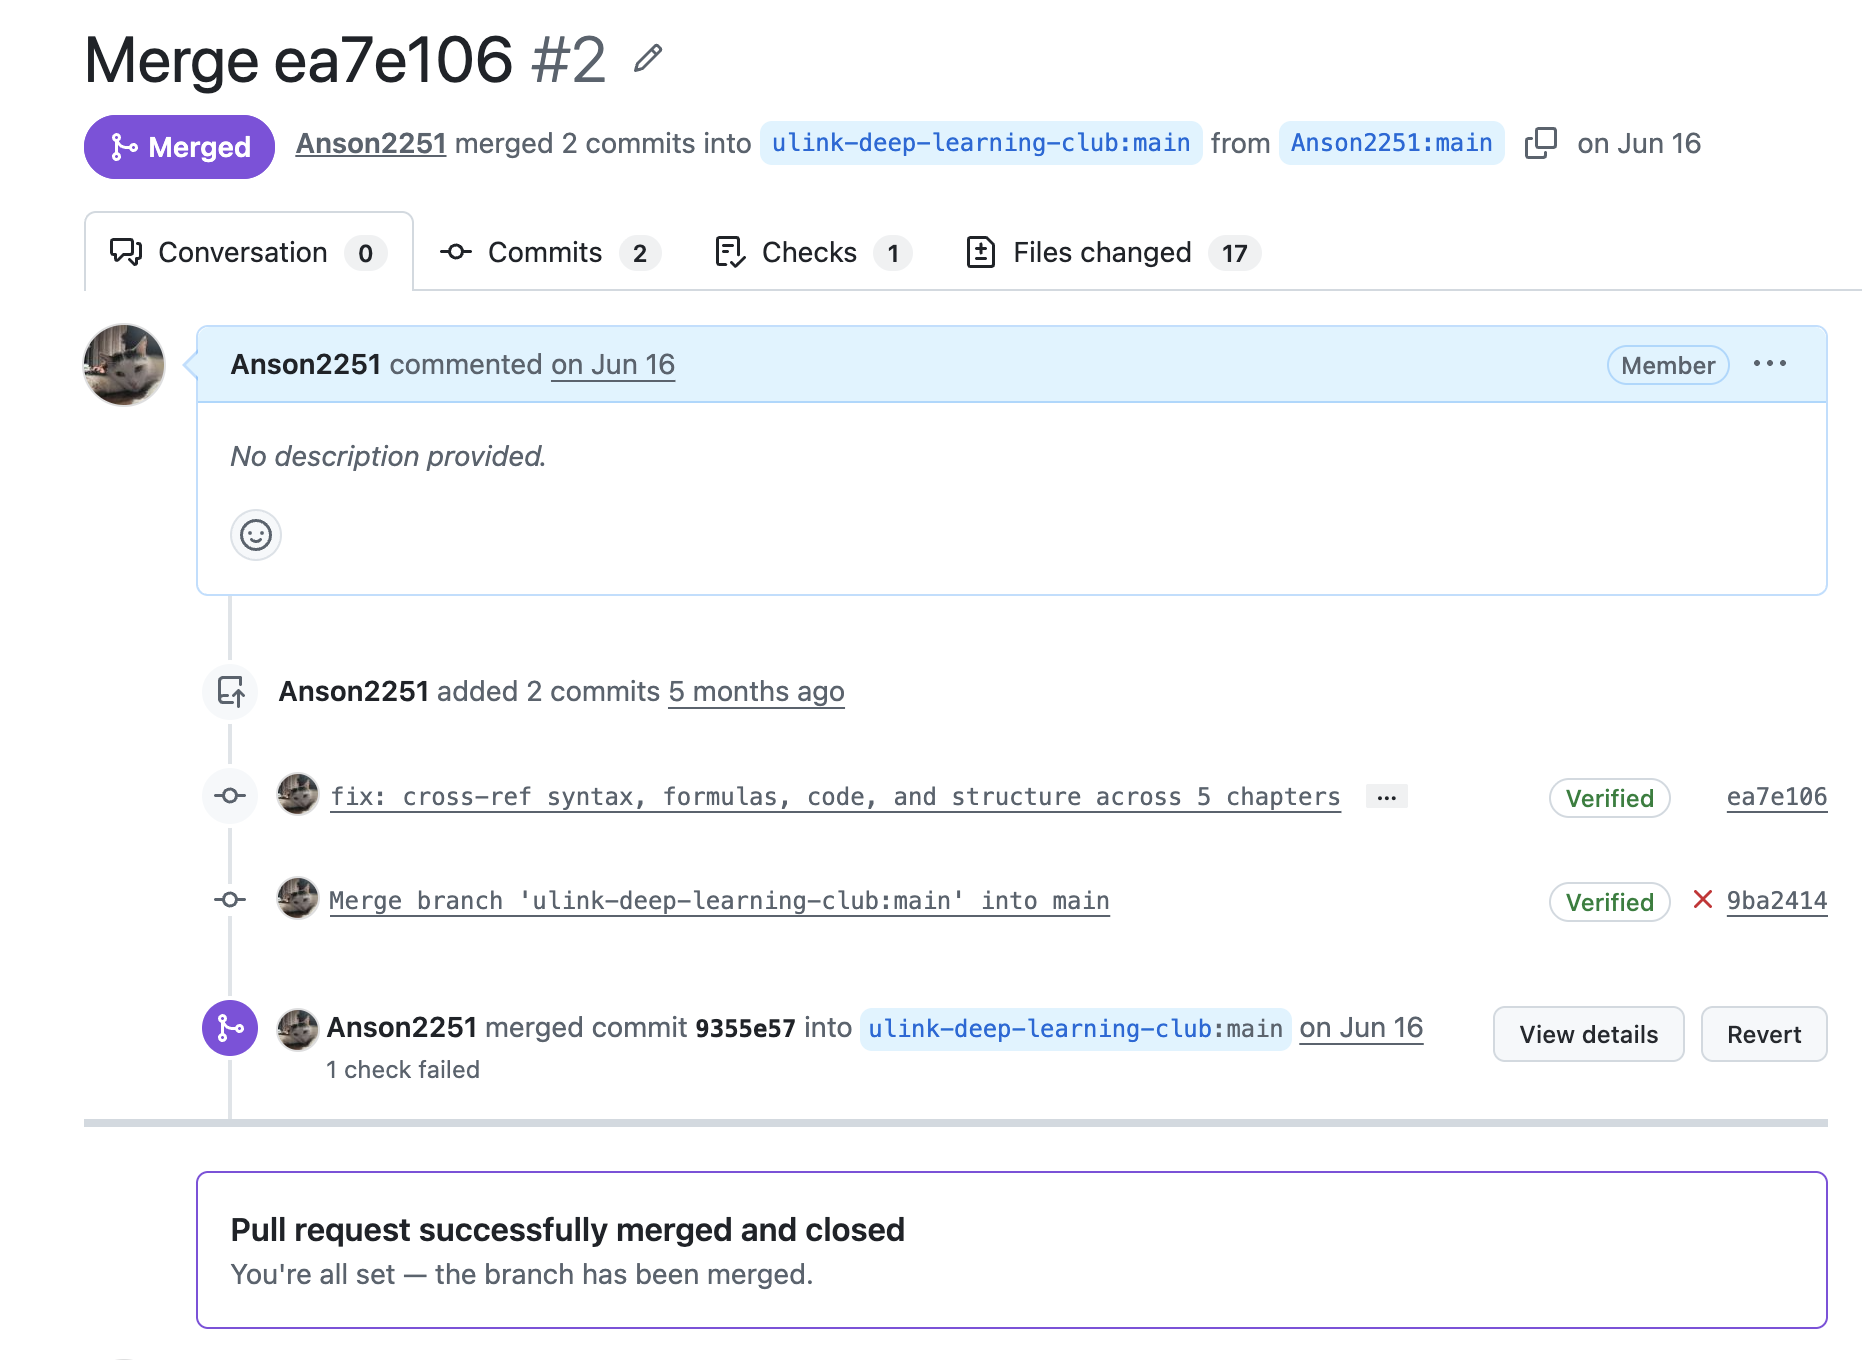
\includegraphics[width=0.85\linewidth]{07-pr-overview.png}
  \caption[GitHub Pull Request 页面，显示 Merged 状态、Conversation、Commits、Checks、Files changed 标签]{PR 页面。Conversation 看讨论，Commits 看提交，Checks 看构建，Files changed 看 diff。}
\end{figure}

标题写清楚改动，正文用这个模板：

\Needspace{5\baselineskip}
\begin{lstlisting}
## 改了什么

把 `source/preface.md` 第 12 行的“机器学系”改成“机器学习”。

## 为什么

原文是错别字，会影响读者理解。

## 怎么验证

- [x] 本地运行 `make html`
- [x] 打开 `build/html/preface.html` 检查文字
- [x] 没有新增构建警告

Closes #12
\end{lstlisting}

最后一行 \code{Closes \#12} 会在 PR 合并后自动关闭对应的 Issue。没有 Issue 就删掉这行。

\begin{tipbox}{Tip}
如果还没改完，可以先点 \code{Create draft pull request}，改完再点 \code{Ready for review}。
\end{tipbox}

\subsection{等检查、改问题、合并}\label{sec:review-and-merge}

PR 打开后，GitHub Actions 会自动构建。绿色的勾表示通过：

\begin{figure}[htbp]
  \centering
  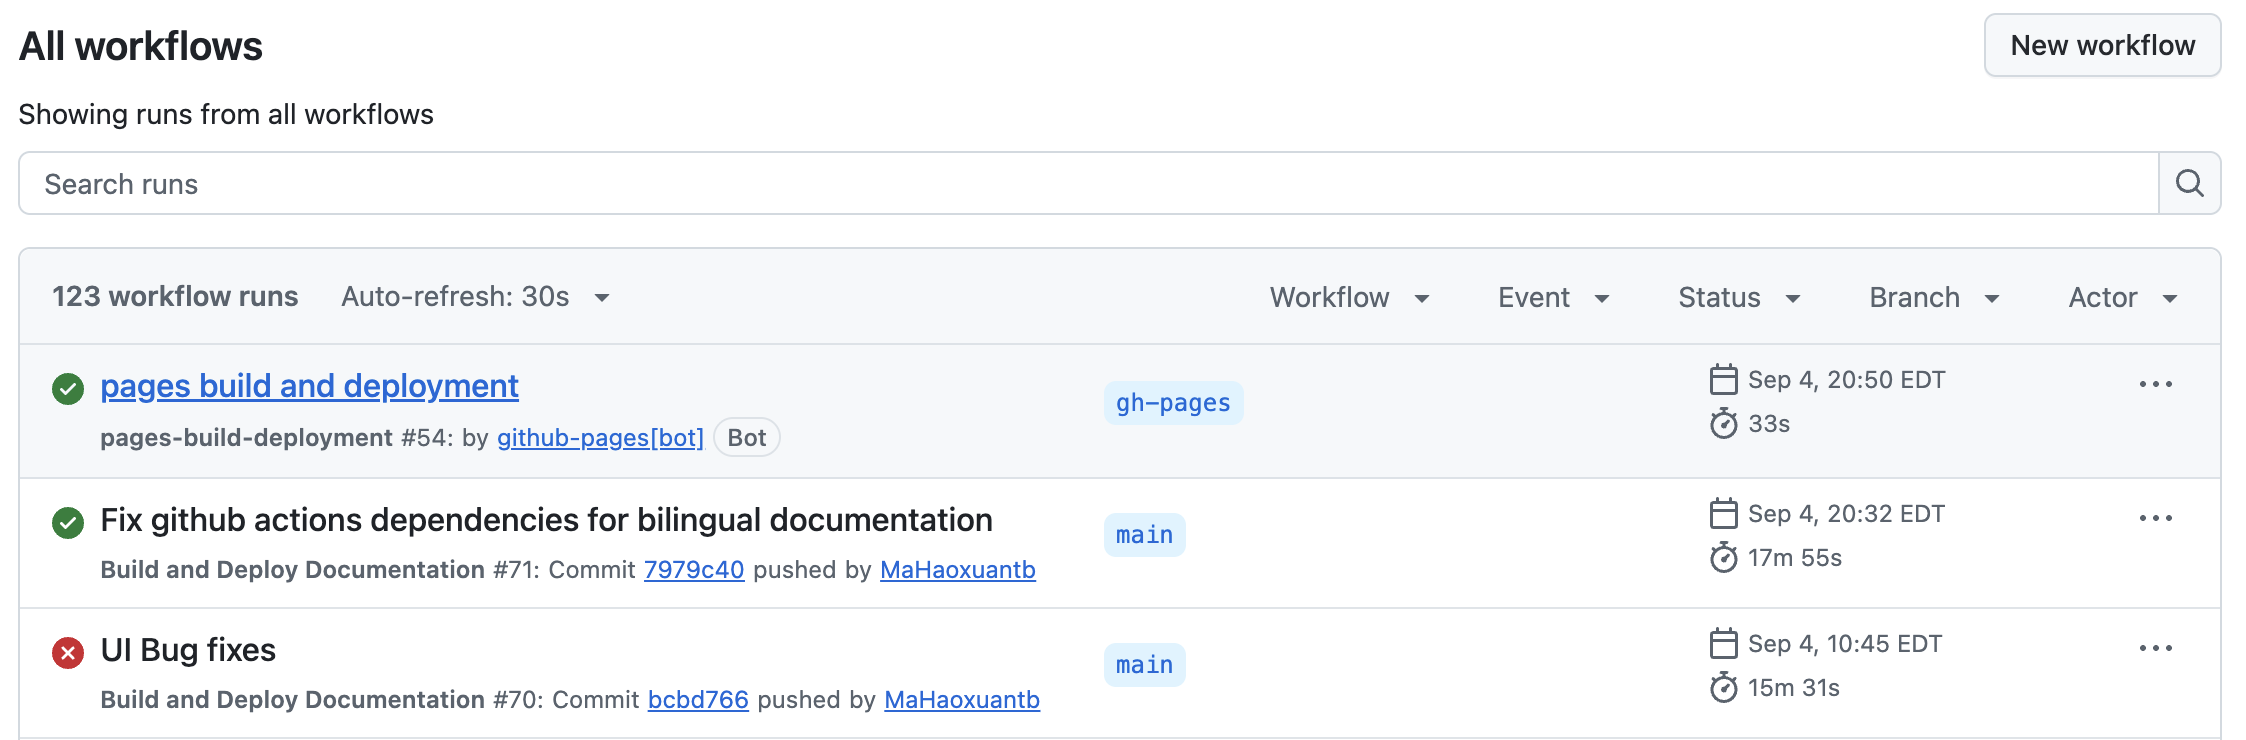
\includegraphics[width=\linewidth]{09-actions.png}
  \caption[GitHub Actions 页面，显示 workflow 运行记录，最近几次是绿色对勾]{Actions 页面。绿色对勾表示构建通过，红色叉号表示失败。}
\end{figure}

点 \code{Checks} 可以看日志。构建失败时，先找第一个 \code{ERROR} 或 \code{WARNING}，那通常才是原因。

审阅者提了修改意见时，不需要新开 PR。在同一个分支继续改，然后：

\Needspace{5\baselineskip}
\begin{lstlisting}[language=bash]
git add <改过的文件>
git commit -m "docs(preface): 根据审阅意见调整措辞"
git push
\end{lstlisting}

PR 会自动更新。\code{Files changed} 页面可以看完整 diff：

\begin{figure}[htbp]
  \centering
  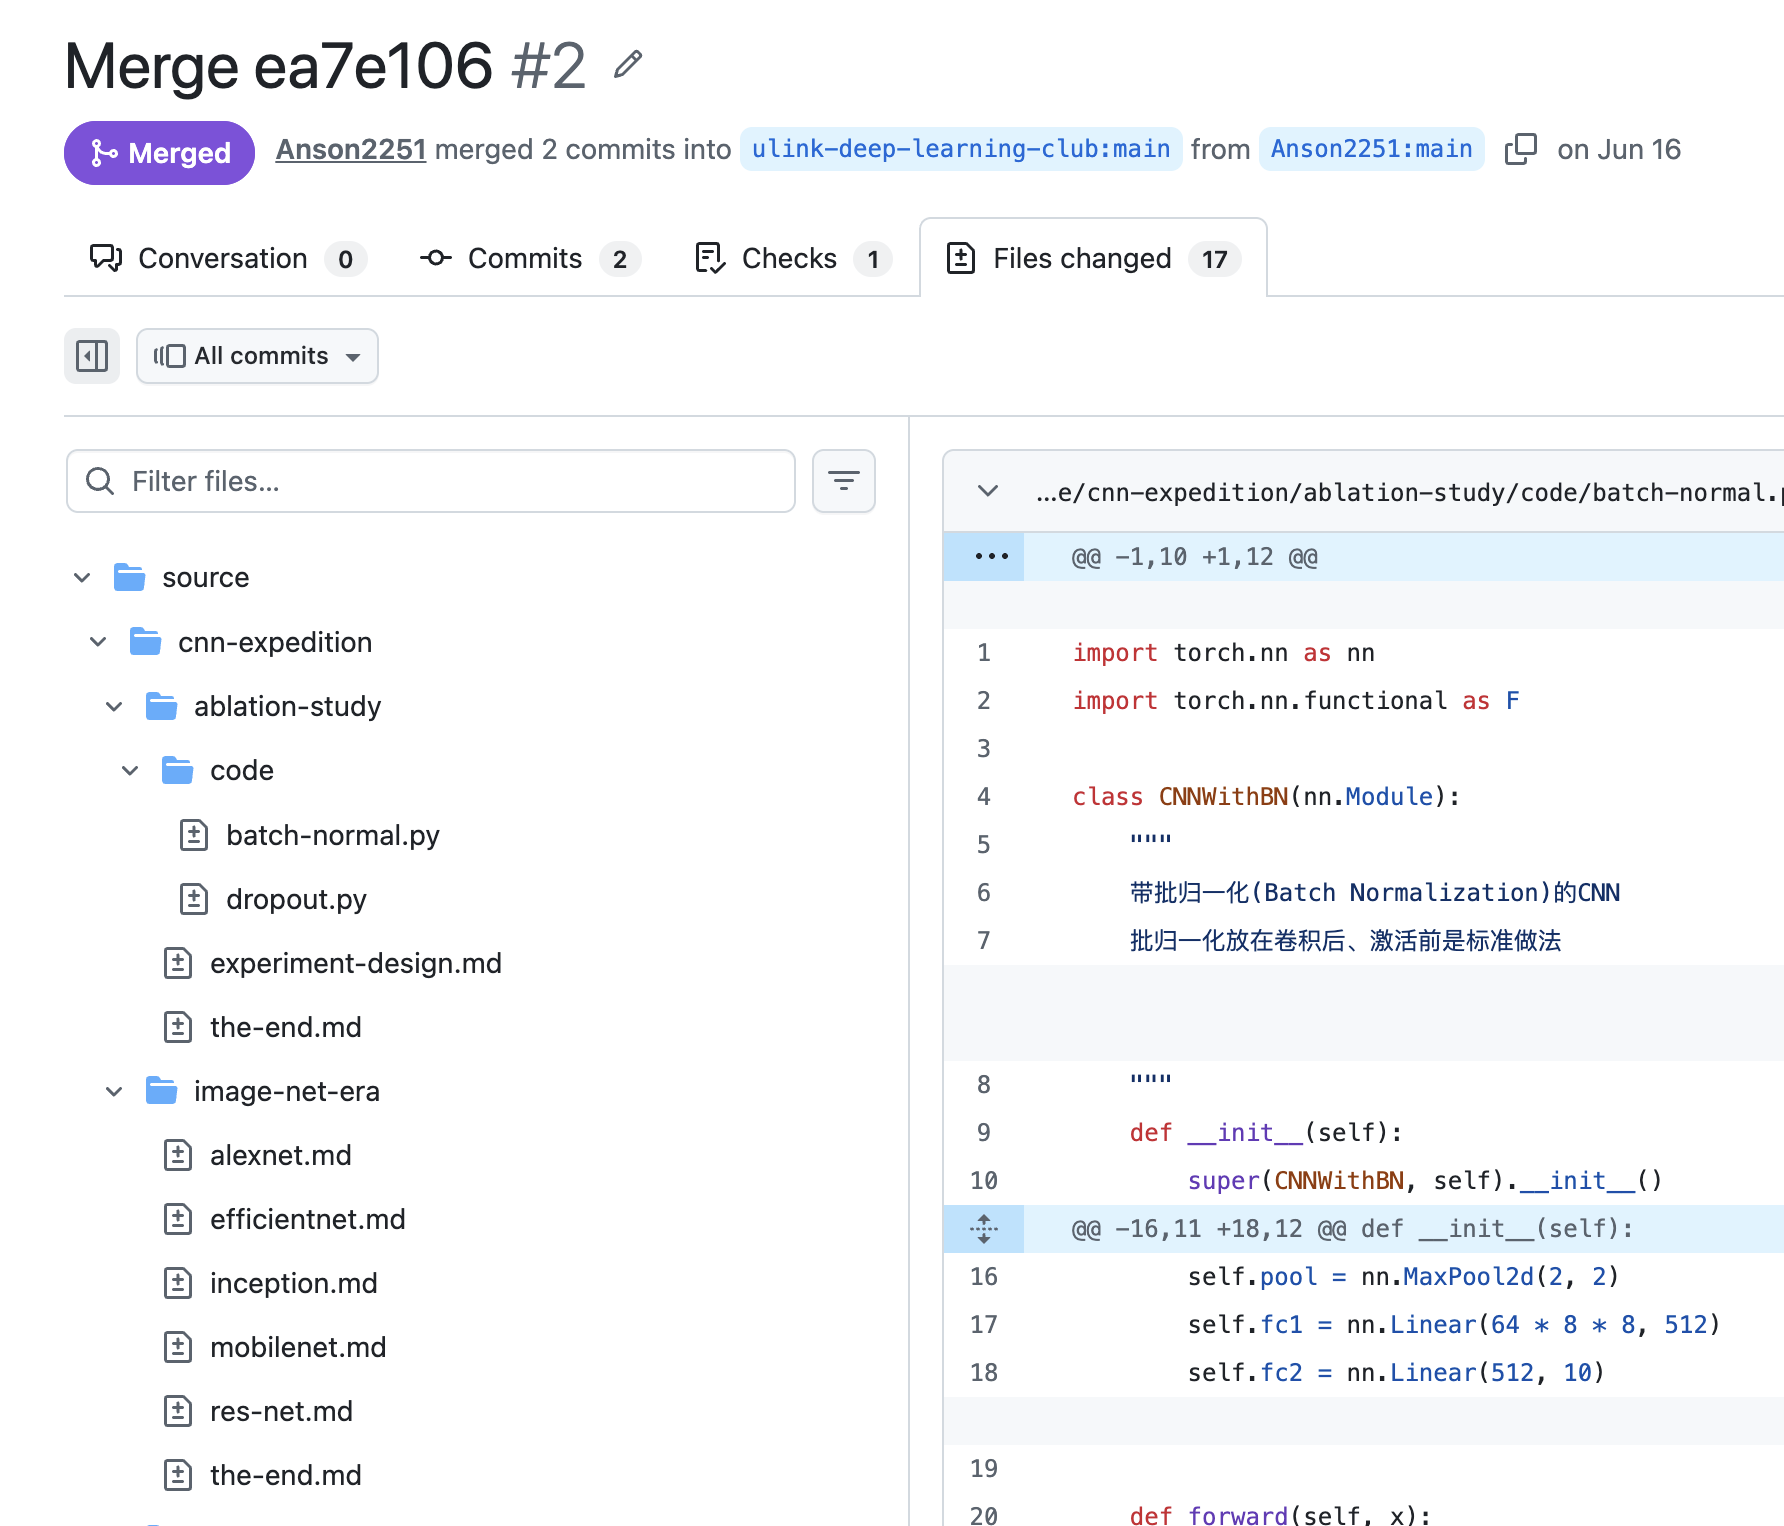
\includegraphics[width=0.82\linewidth]{08-pr-files.png}
  \caption[GitHub Pull Request 的 Files changed 页面，左侧是文件列表，右侧是逐行 diff]{Files changed 页面。左边选文件，右边看逐行改动。}
\end{figure}

审阅者通过后，维护者会点 \code{Merge pull request}。合并完成后可以删除远程分支，GitHub 页面上有按钮。

回到本地，把 \code{main} 更新到最新：

\Needspace{5\baselineskip}
\begin{lstlisting}[language=bash]
git switch main
git pull --ff-only upstream main
git push origin main
\end{lstlisting}

如果你的 fork 页面显示 \code{This branch is behind}，也可以点 \code{Sync fork}。

\clearpage

% ============================== 6. Git 常用操作 ===========================
\section{Git 常用操作}\label{sec:git-commands}

\begin{center}
\small
\begin{tabularx}{\linewidth}{@{}L{5.4cm}Y@{}}
\toprule
目的 & 命令 \\
\midrule
看当前状态 & \code{git status} \\
看未暂存的改动 & \code{git diff} \\
看已暂存的改动 & \code{git diff --staged} \\
暂存一个文件 & \code{git add <文件>} \\
提交 & \code{git commit -m "说明"} \\
推到 fork & \code{git push} \\
拉官方最新 main & \code{git pull --ff-only upstream main} \\
切换分支 & \code{git switch <分支名>} \\
新建并切换分支 & \code{git switch -c <分支名> upstream/main} \\
看提交历史 & \code{git log --oneline --graph} \\
撤销已推送的提交 & \code{git revert <commit>} \\
临时保存未提交的改动 & \code{git stash} \\
取回临时保存的改动 & \code{git stash pop} \\
\bottomrule
\end{tabularx}
\end{center}

\subsection{改错了怎么办}\label{sec:undo}

还没 \code{git add}：

\Needspace{5\baselineskip}
\begin{lstlisting}[language=bash]
git restore <文件>
\end{lstlisting}

已经 \code{git add}，但还没提交：

\Needspace{5\baselineskip}
\begin{lstlisting}[language=bash]
git restore --staged <文件>
\end{lstlisting}

已经提交，但还没推送：

\Needspace{5\baselineskip}
\begin{lstlisting}[language=bash]
git reset --soft HEAD~1
\end{lstlisting}

这会把最后一次提交撤回暂存区，文件内容还在。不要用 \code{git reset --hard}，它会丢掉最后一次提交和未提交的修改。

已经推送的提交不要改写历史。要撤销就运行 \code{git revert <commit>}，它会生成一个反向提交；也可以直接再做一次修正提交。共享分支上执行 \code{git push --force} 会影响别人的工作。

\subsection{遇到冲突}\label{sec:conflicts}

冲突时 Git 会在文件里留下标记：

\Needspace{5\baselineskip}
\begin{lstlisting}
<<<<<<< HEAD
官方仓库现在的内容
=======
你的修改
>>>>>>> fix/typo-preface
\end{lstlisting}

打开文件，保留正确的内容，删掉三行标记，然后：

\Needspace{5\baselineskip}
\begin{lstlisting}[language=bash]
git add <冲突文件>
git rebase --continue
\end{lstlisting}

如果你在做 merge 而不是 rebase，最后一步用 \code{git commit}。不确定时先运行 \code{git status}，它会告诉你当前在 rebase、merge 还是普通状态。冲突太多或 rebase 乱了，可以运行 \code{git rebase --abort} 回到开始前的状态。

% ============================== 7. Markdown 基础 ===========================
\section{Markdown 基础}\label{sec:markdown-basics}

Markdown 用普通字符表示格式。写大部分内容只需要这些语法：

\begin{center}
\small
\begin{tabularx}{\linewidth}{@{}L{5.8cm}Y@{}}
\toprule
写法 & 效果 \\
\midrule
\code{\# 一级标题} & 页面主标题，一个文件通常只有一个 \\
\code{\#\# 二级标题} & 一节 \\
\code{\#\#\# 三级标题} & 一小节 \\
\code{**加粗**} & \textbf{加粗} \\
\code{*斜体*} & \textit{斜体} \\
\code{- 列表项} & 无序列表 \\
\code{1. 列表项} & 有序列表 \\
\code{[文字](https://example.com)} & 链接 \\
\code{\bk 行内代码\bk} & \code{行内代码} \\
\code{> 引用} & 引用块 \\
\code{![说明](图片路径)} & 图片 \\
\code{[\textasciicircum{}1]} & 脚注标记 \\
\bottomrule
\end{tabularx}
\end{center}

代码块用三个反引号包起来，并在开头写语言名：

\Needspace{5\baselineskip}
\begin{lstlisting}
```python
def add(a, b):
    return a + b
```
\end{lstlisting}

表格用竖线分隔：

\Needspace{5\baselineskip}
\begin{lstlisting}
| 方法 | 参数量 | 准确率 |
| --- | --- | --- |
| 全连接 | 235,000 | 98.0% |
| CNN | 61,706 | 99.0% |
\end{lstlisting}

段落之间空一行。标题、列表、代码块、表格的前后也留空行。少一个空行，Sphinx 可能把两段连在一起。

GitHub 的 Markdown 预览能看标题、列表和表格，但看不懂本项目的 \code{\{ref\}}、\code{\{doc\}}、\code{\{note\}} 和 \code{\{literalinclude\}}。最终效果以本地 \code{make html} 为准。

\clearpage

% ============================== 8. MyST 写法 ===============================
\section{本项目的 MyST 写法}\label{sec:myst-syntax}

完整语法在\href{https://github.com/ulink-deep-learning-club/ulink-deeplearningclub-handouts/blob/main/source/appendix/sphinx-guide/index.md}{Sphinx Markdown 语法参考}。

\subsection{文件骨架}\label{sec:file-skeleton}

新章节参照现有文件的结构：

\Needspace{5\baselineskip}
\begin{lstlisting}
(cnn-basics)=
# 卷积神经网络基础

{doc}`cnn-expedition/index`中我们看到了 CNN 的整体位置。本节讨论卷积层如何提取局部特征。

## 历史背景

...

## 主体内容

### 直观理解

...

### 数学表达

...

### 代码实践

...

## 总结

| 概念 | 实践 | 效果 |
| --- | --- | --- |
| 局部感受野 | 3×3 卷积核 | 只看邻居 |

## 下一步

{doc}`le-net`将把这些层组合成完整的 LeNet。
\end{lstlisting}

\code{(cnn-basics)=} 是标签，必须紧贴在标题上一行。标签在同一本书里不能重复。

\subsection{引用其他章节}\label{sec:cross-ref-syntax}

\begin{center}
\small
\begin{tabularx}{\linewidth}{@{}L{2.4cm}L{4.0cm}Y@{}}
\toprule
写法 & 用途 & 例子 \\
\midrule
\code{\{ref\}} & 引用标签 & \code{\{ref\}\bk cnn-basics\bk} \\
\code{\{doc\}} & 引用整篇文档 & \code{\{doc\}\bk cnn-expedition/index\bk} \\
\code{\{cite\}} & 引用文献 & \code{\{cite\}\bk vaswani2017attention\bk} \\
\bottomrule
\end{tabularx}
\end{center}

实际写法：

\Needspace{5\baselineskip}
\begin{lstlisting}
回顾{ref}`inductive-bias`中的讨论。

下一节见{doc}`le-net`。

Transformer 的原始论文见{cite}`vaswani2017attention`。
\end{lstlisting}

\code{\{doc\}} 的路径相对于 \code{source/}，不带 \code{.md}。\code{\{ref\}} 只写标签名，不带括号。

\subsection{提示框}\label{sec:admonitions}

\Needspace{5\baselineskip}
\begin{lstlisting}
```{note}
这是一条补充说明。
```

```{tip}
这是一条建议。
```

```{warning}
这里要提醒读者注意。
```
\end{lstlisting}

可用的类型有 \code{note}、\code{tip}、\code{warning}、\code{caution}、\code{danger}、\code{important}、\code{hint}、\code{attention}、\code{error}。

\subsection{Mermaid 图}\label{sec:mermaid-syntax}

项目里的 Mermaid 常用波浪线包起来，避免和外层代码块冲突：

\Needspace{5\baselineskip}
\begin{lstlisting}
~~~{mermaid}
flowchart LR
    A["输入图像"] --> B["卷积层"]
    B --> C["池化层"]
    C --> D["全连接层"]
~~~
\end{lstlisting}

Mermaid 适合画流程图、结构图和时间线。复杂网络结构用 TikZ，语法在\href{https://github.com/ulink-deep-learning-club/ulink-deeplearningclub-handouts/blob/main/source/appendix/sphinx-guide/index.md}{Sphinx Markdown 语法参考}。

截图和照片放在 Markdown 文件旁边或 \code{\_static/images/}，用相对路径引用。图片宽度控制在 400 到 600 px，并写清替代文字（alt text）。

\subsection{数学公式}\label{sec:math-syntax}

行内公式用美元符号包住：

\Needspace{5\baselineskip}
\begin{lstlisting}
卷积输出的大小是 $W_{out} = W_{in} - k + 1$。
\end{lstlisting}

独立公式用两个美元符号：

\Needspace{5\baselineskip}
\begin{lstlisting}
$$
Y[i,j] = \sum_{u=0}^{k-1}\sum_{v=0}^{k-1} X[i+u,j+v] \cdot K[u,v]
$$
\end{lstlisting}

行间公式前后留空行。公式里不要用中文标点。

\subsection{代码}\label{sec:code-syntax}

短代码可以直接写在正文里。长代码放在章节的 \code{code/} 目录，用 \code{literalinclude} 引用：

\Needspace{5\baselineskip}
\begin{lstlisting}
```{literalinclude} code/batch-normal.py
:language: python
:linenos:
:caption: 带 BatchNorm 的 CNN
```
\end{lstlisting}

这样做有两个好处：代码文件可以被单独运行，MyST 也不会把代码里的花括号当成指令。

代码注释写清楚维度、参数计算和对应的理论。项目要求比较细，例子：

\Needspace{5\baselineskip}
\begin{lstlisting}[language=python]
def forward(self, x):
    # 输入 x: [batch, 1, 28, 28]
    x = self.conv1(x)  # 1→32 通道，3×3 卷积，输出 [batch, 32, 26, 26]
    x = F.relu(x)      # 非线性激活
    x = self.pool(x)   # 2×2 最大池化，输出 [batch, 32, 13, 13]
    return x
\end{lstlisting}

\subsection{表格}\label{sec:table-syntax}

普通 Markdown 表格够用。需要多级表头或把指令嵌进表格时，用 \code{\{list-table\}}：

\Needspace{5\baselineskip}
\begin{lstlisting}
```{list-table} 全连接与 CNN 对比
:header-rows: 1

* - 模型
  - 参数量
  - 准确率
* - 全连接
  - 235,000
  - 98.0%
* - CNN
  - 61,706
  - 99.0%
```
\end{lstlisting}

\subsection{文献}\label{sec:bibliography-syntax}

所有条目放在 \code{source/references.bib}，key 用“作者姓氏 + 年份 + 关键词”：

\Needspace{5\baselineskip}
\begin{lstlisting}
@inproceedings{vaswani2017attention,
  title={Attention is all you need},
  author={Vaswani, Ashish and others},
  booktitle={Advances in Neural Information Processing Systems},
  volume={30},
  year={2017}
}
\end{lstlisting}

正文用 \code{\{cite\}} 引用。文件末尾加参考文献列表：

\Needspace{5\baselineskip}
\begin{lstlisting}
## 参考文献

```{bibliography}
:filter: docname in docnames
```
\end{lstlisting}

\code{:filter: docname in docnames} 只列出当前页面实际引用过的条目。不要把所有文献都列在每一页。

\subsection{目录树}\label{sec:toctree-syntax}

每个章节的 \code{index.md} 用隐藏的 \code{\{toctree\}} 定义阅读顺序：

\Needspace{5\baselineskip}
\begin{lstlisting}
```{toctree}
:maxdepth: 2
:hidden:

introduction
cnn-basics
le-net
the-end
```
\end{lstlisting}

条目是相对路径，不带 \code{.md}。新增文件后，记得把它加进对应章节的 \code{index.md}，否则读者在网页导航里找不到。

% ============================== 9. 写作要求 ================================
\section{写作要求}\label{sec:writing-rules}

项目的写作约定总结如下，完整语法见\href{https://github.com/ulink-deep-learning-club/ulink-deeplearningclub-handouts/blob/main/source/appendix/sphinx-guide/index.md}{Sphinx Markdown 语法参考}。最常用的几条：

\begin{center}
\small
\begin{tabularx}{\linewidth}{@{}L{4.2cm}Y@{}}
\toprule
要求 & 做法 \\
\midrule
先建立直觉 & 先用生活类比或几何直觉说明“为什么”，再给公式 \\
用对比帮助理解 & 用表格比较全连接与 CNN、RNN 与 Transformer \\
用数字支撑 & 写清参数量、准确率、时间，数字用千分位 \\
代码带注释 & 注释写维度、参数计算和对应的理论 \\
建立知识网络 & 每个主要概念至少有一个 \code{\{ref\}} 或 \code{\{doc\}} 链接 \\
交代历史 & 提到提出者、年份和原始论文 \\
结尾给下一步 & 总结本节，再链接到下一节 \\
\bottomrule
\end{tabularx}
\end{center}

一个概念出现时，先链接到它的定义或前置章节。比如第一次提到反向传播，就用 \code{\{ref\}} 链接到对应标签，读者可以跳回去补基础。

章节结构按现有文件来：\code{index.md} 放概览和 toctree，中间放内容文件，最后用 \code{the-end.md} 收尾。不要单独新建一个没有 toctree 的目录。

术语要统一。同一个概念第一次出现时给出英文对照，后面用同一个中文译名。数字用千分位，百分比保留一位小数。

\clearpage

% ============================== 10. 代码贡献 ===============================
\section{代码贡献}\label{sec:code-contrib}

改文字不需要会 Python。只有修改 \code{code/} 里的示例或新增代码时，才需要运行 Python。

正文里的代码和 \code{code/} 目录里的脚本是两回事。正文用 \code{literalinclude} 引用脚本，读者看到的是同一份代码。

新增或修改代码时注意这些：

\begin{itemize}[leftmargin=1.8em,itemsep=2pt]
  \item 脚本放在对应章节的 \code{code/} 目录，文件名用能看懂的小写加连字符。
  \item 代码要能单独运行。需要数据或 GPU 时，在文件开头写清依赖和运行方式。
  \item 依赖变化时更新 \code{pyproject.toml} 和 \code{uv.lock}，在 PR 里说明为什么加。
  \item 不要提交数据集、模型权重、训练日志、\code{.pth} 或 \code{.ckpt} 文件。
  \item 不要提交 API key、密码、token、个人路径和内网地址。
  \item 不能运行代码时，在 PR 里写“未运行，缺少 PyTorch/GPU”，不要假装跑过。
\end{itemize}

终端最常用的命令：

\begin{center}
\small
\begin{tabularx}{\linewidth}{@{}L{5.6cm}Y@{}}
\toprule
命令 & 作用 \\
\midrule
\code{pwd} & 显示当前目录 \\
\code{ls} & 列出文件 \\
\code{cd <目录>} & 进入目录 \\
\code{cd ..} & 回到上一级 \\
\code{mkdir <目录>} & 新建目录 \\
\code{cp <源> <目标>} & 复制文件 \\
\code{mv <源> <目标>} & 移动或重命名 \\
\code{rm <文件>} & 删除文件，删了不能恢复 \\
\code{cat <文件>} & 显示文件内容 \\
\code{grep -rn "文字" .} & 在当前目录递归搜索文字 \\
\bottomrule
\end{tabularx}
\end{center}

Python 报错时，先看 traceback 的最后一行。它通常写着错误类型和原因，例如\newline\code{ModuleNotFoundError:}\allowbreak\ \code{No module named}\allowbreak\ \code{'torch'}。把完整错误贴到 Issue 或聊天里，比只说“跑不起来”更容易得到帮助。

\clearpage

% ============================== 11. 翻译贡献 ===============================
\section{翻译贡献}\label{sec:translation}

中文 Markdown 是唯一的内容源。英文翻译放在 \code{source/locale/en/LC\_MESSAGES/} 下，和中文文件路径对应。

改中文后，需要刷新翻译目录：

\Needspace{5\baselineskip}
\begin{lstlisting}[language=bash]
sphinx-build -W --keep-going -b gettext source build/i18n/gettext
sphinx-intl update -p build/i18n/gettext -l en
python scripts/check-i18n.py
\end{lstlisting}

规则在\href{https://github.com/ulink-deep-learning-club/ulink-deeplearningclub-handouts/blob/main/docs/i18n/AGENT_GUIDE.md}{本地化工作指南}，术语在\href{https://github.com/ulink-deep-learning-club/ulink-deeplearningclub-handouts/blob/main/docs/i18n/glossary.md}{术语表}。几条容易犯的错：

\begin{itemize}[leftmargin=1.8em,itemsep=2pt]
  \item 不要新建一棵英文 Markdown 源树。
  \item 不要改 \code{\{doc\}}、\code{\{ref\}} 的标签、引用 key、URL、公式、文件名和代码逻辑。
  \item 不要把中文 \code{msgid} 直接复制成 \code{msgstr} 来假装翻译完成。
  \item 翻译完要检查渲染后的 HTML，表格和 TikZ 里的文字可能不会被 gettext 提取。
  \item 一次只做一个顶层章节，方便英文审校者审阅。
  \item 不要提交 \code{build/}、\code{.pot} 或 \code{.mo} 文件，只提交 \code{.po} 目录。
\end{itemize}

完整检查：

\Needspace{5\baselineskip}
\begin{lstlisting}[language=bash]
python scripts/check-i18n.py --require-complete --prefix math-fundamentals
bash scripts/build-i18n-site.sh --html-only
\end{lstlisting}

\section{提交前检查}\label{sec:preflight}

\begin{itemize}[label={\small$\square$},leftmargin=1.7em,itemsep=3pt]
  \item \code{git status} 里只有你打算提交的文件
  \item \code{git diff} 里没有误删、个人路径、密钥或无关格式改动
  \item \code{make html} 能通过，新增的 \code{WARNING} 已处理
  \item 新增的 \code{\{ref\}} 和 \code{\{doc\}} 都能跳转
  \item 代码能运行，或已在 PR 里说明未运行的原因
  \item Mermaid/TikZ 能渲染，或已说明缺少依赖
  \item 新文件已加入对应章节的 \code{index.md} 的 toctree
  \item 提交信息说清了改什么
  \item PR 描述包含原因和验证方式
  \item 翻译改动已运行 \code{check-i18n.py}
\end{itemize}

\clearpage

% ============================== 13. 常见问题 ===============================
\section{常见问题}\label{sec:faq}

{\small
\setlength{\tabcolsep}{4pt}
\begin{longtable}{@{}L{4.2cm}L{4.1cm}L{6.6cm}@{}}
\toprule
现象 & 原因 & 处理 \\
\midrule
\endhead
\code{fatal: not a git repository} & 终端不在仓库目录 & \code{cd} 到仓库根目录 \\
\code{remote origin already exists} & 已经有同名远程 & \code{git remote set-url origin <地址>} \\
\code{Updates were rejected} & 远程有你本地没有的提交 & \code{git pull --rebase}，解决冲突后再 push \\
\code{CONFLICT (content)} & 同一段文字被两边修改 & 打开文件改掉冲突标记，\code{git add} 后继续 \\
\code{make: command not found} & Windows 或环境没装 make & 用 \code{make.bat html}，或改用 WSL \\
\code{uv: command not found} & 没装 uv & 用 \code{python3 -m venv} 和 \code{pip install -e .} \\
\code{No module named sphinx} & 虚拟环境没激活 & Linux/macOS 用 \code{source .venv/bin/activate}，Windows 用 \code{.venv\textbackslash{}Scripts\textbackslash{}activate} \\
Mermaid 图不显示 & 没装 Chromium 或 mermaid-cli & 安装依赖，或先接受图表缺失继续改文字 \\
中文 PDF 显示方框 & 缺中文字体 & 安装 Noto Sans CJK，见 build-docs 附录 \\
\code{\{ref\}} 找不到 & 标签拼错或没定义 & 检查标签拼写和位置，重新构建看警告 \\
\code{\{doc\}} 找不到 & 路径多了 \code{.md} 或写错层级 & 路径相对 \code{source/}，不带扩展名 \\
页面没更新 & 浏览器缓存或构建目录旧 & 刷新，必要时 \code{rm -rf build/html} 重构建 \\
误提交了 \code{build/} & \code{git add .} 带进了产物 & \code{git rm -r --cached build}，它已在 \code{.gitignore} 里 \\
误提交了密钥 & 文件里有 token 或密码 & 立刻撤销密钥，通知维护者，仅删文件不够 \\
\bottomrule
\end{longtable}
}

命令报错时，先判断是哪一步出的问题：

\begin{figure}[H]
  \centering
  \begin{tikzpicture}
    \node[flowin] (A) at (0,0) {命令报错};
    \node[decision] (B) at (0,-1.7) {哪一步};
    \node[flow,text width=4.2cm,font=\footnotesize\sffamily] (C) at (-5.2,-3.9) {读输出的第一行和最后一行};
    \node[flow,text width=4.2cm,font=\footnotesize\sffamily] (D) at (0,-3.9) {搜索第一个 ERROR 或 WARNING};
    \node[flow,text width=4.2cm,font=\footnotesize\sffamily] (E) at (5.2,-3.9) {看 traceback 最后一行};
    \node[flow] (F) at (0,-5.7) {复制完整命令和错误};
    \node[flowout] (G) at (0,-7.2) {贴到 Issue、PR 评论或群里};

    \draw[edge] (A) -- (B);
    \draw[edge] (B) -- node[elabel,above]{git} (C);
    \draw[edge] (B) -- node[elabel,right]{make 或 sphinx} (D);
    \draw[edge] (B) -- node[elabel,above]{python} (E);
    \draw[edge] (C) -- (F);
    \draw[edge] (D) -- (F);
    \draw[edge] (E) -- (F);
    \draw[edge] (F) -- (G);
  \end{tikzpicture}
  \caption{报错时的排查顺序}
\end{figure}

求助时写清四件事：你运行了什么命令、完整错误是什么、操作系统是什么、你已经试过什么。截图可以，但文字更方便别人搜索和复制。

% ============================== 14. 术语表 =================================
\section{术语表}\label{sec:glossary}

{\small
\setlength{\tabcolsep}{4pt}
\begin{longtable}{@{}L{3.0cm}L{2.4cm}L{9.6cm}@{}}
\toprule
英文 & 中文 & 说明 \\
\midrule
\endhead
repository & 仓库 & 带历史记录的项目目录 \\
fork & 派生副本 & 复制到你自己账号下的仓库 \\
clone & 克隆 & 把远程仓库下载到本地 \\
branch & 分支 & 一条独立的修改线 \\
commit & 提交 & 一次有说明的修改记录 \\
push & 推送 & 把本地提交上传到远程 \\
pull & 拉取 & 把远程更新下载并合并到本地 \\
remote & 远程 & 另一份仓库的地址 \\
upstream & 上游 & 本项目中指官方仓库 \\
origin & 源 & 本项目中指你的 fork \\
staging area & 暂存区 & 准备写进下一次提交的改动 \\
merge & 合并 & 把一条分支接回另一条 \\
conflict & 冲突 & 两边改了同一处，需要手动选择 \\
Pull Request & 拉取请求 & 请求官方仓库合并你的分支 \\
Issue & 议题 & 讨论问题或提出修改建议 \\
CI & 持续集成 & 自动构建和检查，本项目用 GitHub Actions \\
\bottomrule
\end{longtable}
}

\clearpage

% ============================== 15. 接下来做什么 ===========================
\section{接下来做什么}\label{sec:next-steps}

从一个具体的文件开始。打开 \href{https://github.com/ulink-deep-learning-club/ulink-deeplearningclub-handouts/blob/main/source/preface.md}{\code{source/preface.md}}，读一遍，找一句可以写得更清楚的话，或者找一个错别字。按第~\ref{sec:web-edit}~节在网页上改掉它，走一次完整的 PR 流程。

第二次可以选一个规模不大的 Issue，或者给某一节补一张 Mermaid 图。改之前先读相邻章节和\href{https://github.com/ulink-deep-learning-club/ulink-deeplearningclub-handouts/blob/main/source/appendix/sphinx-guide/index.md}{Sphinx Markdown 语法参考}，确认术语和结构一致。提交 PR 时写清你运行过的命令和看到的页面，审阅者会更快理解你的改动。

\section{相关链接}\label{sec:links}

\begin{itemize}[leftmargin=1.8em,itemsep=2pt]
  \item \href{https://github.com/ulink-deep-learning-club/ulink-deeplearningclub-handouts}{项目仓库}
  \item \href{https://github.com/ulink-deep-learning-club/ulink-deeplearningclub-handouts/blob/main/README.md}{项目 README}
  \item \href{https://ulink-deep-learning-club.github.io/ulink-deeplearningclub-handouts/}{在线文档}
  \item \href{https://github.com/ulink-deep-learning-club/ulink-deeplearningclub-handouts/issues}{Issue 列表}
  \item \href{https://github.com/ulink-deep-learning-club/ulink-deeplearningclub-handouts/pulls}{Pull requests}
  \item \href{https://github.com/ulink-deep-learning-club/ulink-deeplearningclub-handouts/actions}{Actions 构建记录}
  \item \href{https://github.com/ulink-deep-learning-club/ulink-deeplearningclub-handouts/blob/main/source/appendix/sphinx-guide/index.md}{Sphinx Markdown 语法参考}
  \item \href{https://github.com/ulink-deep-learning-club/ulink-deeplearningclub-handouts/blob/main/source/appendix/build-docs.md}{本地构建说明}
  \item \href{https://github.com/ulink-deep-learning-club/ulink-deeplearningclub-handouts/blob/main/docs/i18n/AGENT_GUIDE.md}{本地化工作指南}
  \item \href{https://github.com/ulink-deep-learning-club/ulink-deeplearningclub-handouts/blob/main/docs/i18n/glossary.md}{术语表}
\end{itemize}

\end{document}
